\documentclass[aspectratio=169,11pt]{beamer}
\usepackage[utf8]{inputenc}
\usepackage{amsmath, amssymb, bm}
\usepackage{booktabs}
\usepackage{listings}
\usepackage{graphicx}

% --- Universidad de Antioquia (UdeA) Custom Theme Setup ---
\definecolor{UdeAGreen}{HTML}{006241}
\definecolor{UdeAGold}{HTML}{D4AF37}
\definecolor{Charcoal}{HTML}{2B2B2B}
\definecolor{LightBg}{HTML}{F8F9FA}

\setbeamercolor{palette primary}{bg=UdeAGreen, fg=white}
\setbeamercolor{palette secondary}{bg=UdeAGreen, fg=white}
\setbeamercolor{structure}{fg=UdeAGreen}
\setbeamercolor{background canvas}{bg=LightBg}
\setbeamercolor{text}{fg=Charcoal}

% --- Block Style Customization ---
\setbeamercolor{block title}{bg=UdeAGreen, fg=white}
\setbeamercolor{block body}{bg=white, fg=Charcoal}
\setbeamercolor{block title example}{bg=UdeAGold, fg=Charcoal}
\setbeamercolor{block body example}{bg=white, fg=Charcoal}

% --- Header/Footer Customization ---
\setbeamertemplate{headline}{}
\setbeamertemplate{footline}{%
    \leavevmode%
    \begin{beamercolorbox}[wd=\paperwidth,ht=2.5ex,dp=1.125ex,leftskip=.3cm,rightskip=.3cm]{palette primary}%
        \small Universidad de Antioquia -- Faculty of Engineering \hfill Module 1: Perturbations \hfill \insertframenumber/\inserttotalframenumber%
    \end{beamercolorbox}%
}
\setbeamertemplate{navigation symbols}{}

% --- Code Presentation Configuration ---
\lstset{
    backgroundcolor=\color{LightBg},
    basicstyle=\tiny\ttfamily\color{Charcoal},
    breaklines=true,
    keywordstyle=\color{UdeAGreen}\bfseries,
    commentstyle=\color{gray},
    stringstyle=\color{UdeAGold},
    frame=single
}

% --- THEME AND FONT ---
\usetheme{Madrid}                % Sets layout (e.g., Madrid, Frankfurt, Boadilla)
\usefonttheme{professionalfonts} % Ensures equations render accurately

% Positions logo in the upper right corner
\logo{\vspace{-0.2cm}\hfill
\includegraphics[width=1cm]{Images/UdeA+simplificado+Negro_Smaller.png}\hspace{0.1cm}}

\title[Astrodynamics Module]{Astrodynamics Module Content} 
\author{Juan Francisco Puerta Ibarra}
\institute{Aerospace Engineering}
\date{Semester 2026-2}
\titlegraphic{
\includegraphics[width=3cm]{Images/UdeA+simplificado+Negro_Smaller.png}}

\begin{document}

% --- TITLE SLIDE ---
\begin{frame}[plain]
    \titlepage
\end{frame}

% --- MODULE OVERVIEW ---
\begin{frame}{Review: Two Body Problem}
    \begin{block}{Module 1. Orbital Perturbations (The "Real" Solar System)}
        The \textbf{gravitational two-body problem} concerns the motion of two point particles that interact only with each other, due to gravity. This means that influences from any third body are neglected.
    \end{block}
    
    \vspace{0.2cm}
    \textbf{Weekly Roadmap and Mathematical Benchmarks:}
    \begin{itemize}
        \item{Week 1:} Foundations of Non-Keplerian Acceleration.
        \item{Week 2:} Zonal Harmonics and the Geopotential Spectrum.
        \item{Week 3:} Advanced Constrained Orbit Design.
        \item{Week 4:} Non-Conservative Force Coupling and Lifetime Loops.
    \end{itemize}
\end{frame}

\begin{frame}{Review: Two Body Problem}
    \vspace*{-0.3cm}
    \begin{columns}[T]
        \begin{column}{0.30\textwidth}
            \small
            \begin{exampleblock}{Module 1. Orbital Perturbations (The "Real" Solar System)}
                A little review from before… Two-Body Problem
            \end{exampleblock}
        \end{column}
        \begin{column}{0.70\textwidth}
            \centering
            \vspace{0.1cm}
            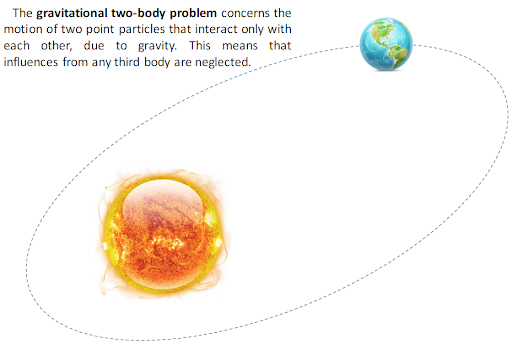
\includegraphics[width=\linewidth,height=0.70\textheight,keepaspectratio]{Images/Earth_sun.png}
        \end{column}
    \end{columns}
\end{frame}

\begin{frame}{Review: Two Body Problem}
    \vspace*{-0.3cm}
    \begin{columns}[T]
        \begin{column}{0.30\textwidth}
            \small
            \begin{exampleblock}{Module 1. Orbital Perturbations (The "Real" Solar System)}
                A little review from before… Two-Body Problem
            \end{exampleblock}
        \end{column}
        \begin{column}{0.70\textwidth}
            \centering
            \vspace{0.1cm}
            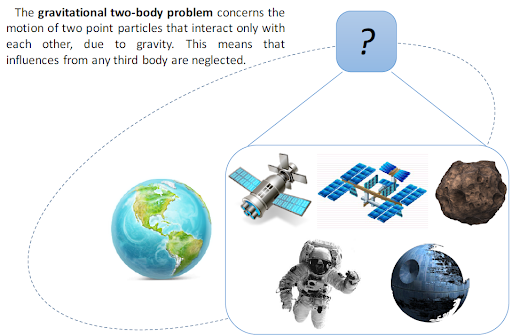
\includegraphics[width=\linewidth,height=0.70\textheight,keepaspectratio]{Images/Earth to sc.png}
        \end{column}
    \end{columns}
\end{frame}

% --- MODULE OVERVIEW ---
\begin{frame}{Review: Reference Frames*}
    \footnotesize
    \begin{block}{Inertial reference frames}
        \begin{itemize}
            \item A coordinate system that is either at rest or moving at a constant velocity.
            \item Newton's laws are valid only in inertial reference frames.
        \end{itemize}
    \end{block}
    
    \vspace{0.2cm}
    \begin{figure}
        \centering
        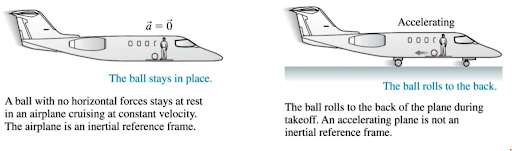
\includegraphics[width=0.75\textwidth]{Images/frames.png}
    \end{figure}
\end{frame}

\begin{frame}{Review: Two Body Problem}
    \begin{figure}
        \centering
        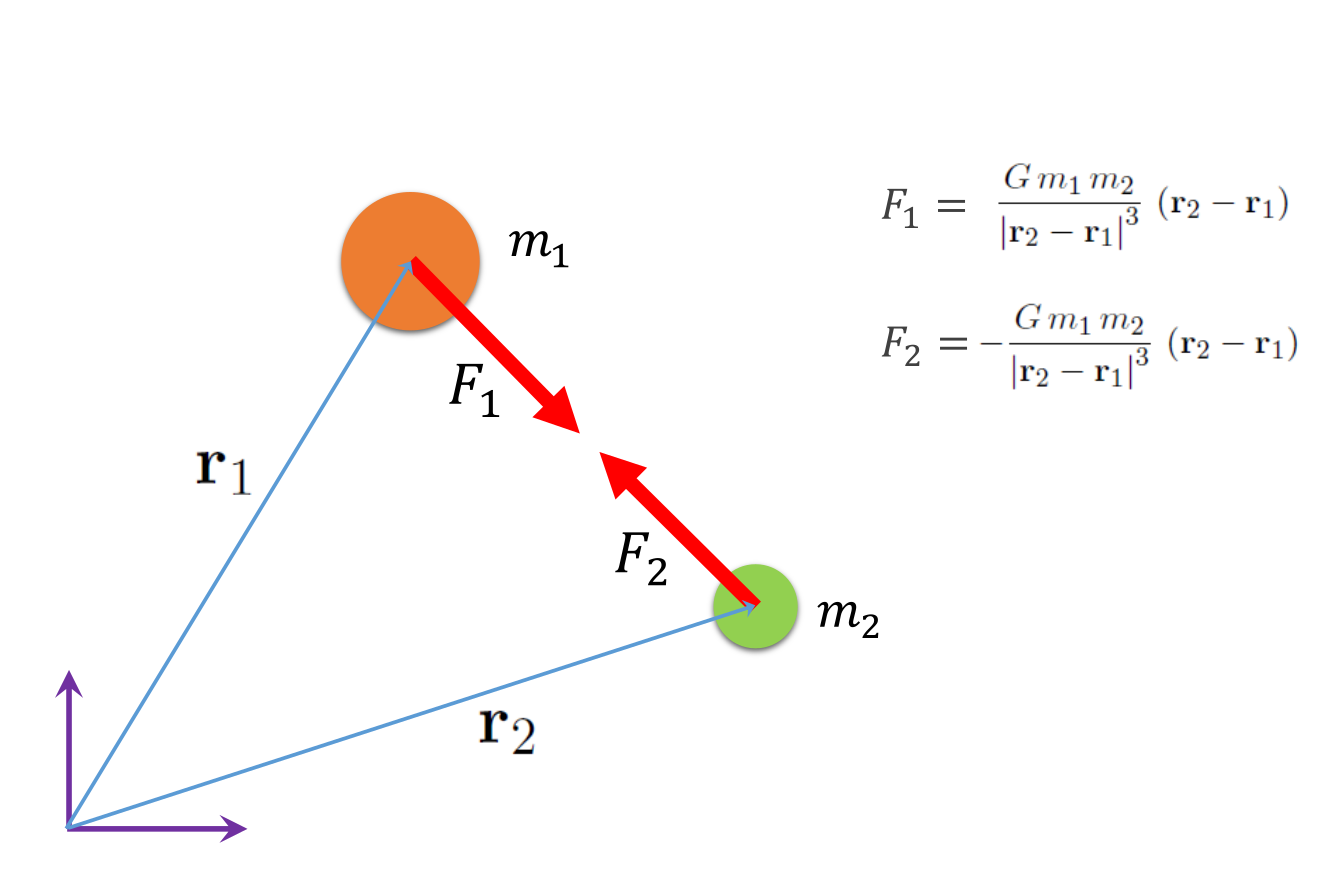
\includegraphics[width=0.75\textwidth]{Images/TBP1.png}
    \end{figure}
\end{frame}

\begin{frame}{Review: Two Body Problem}
    \begin{figure}
        \centering
        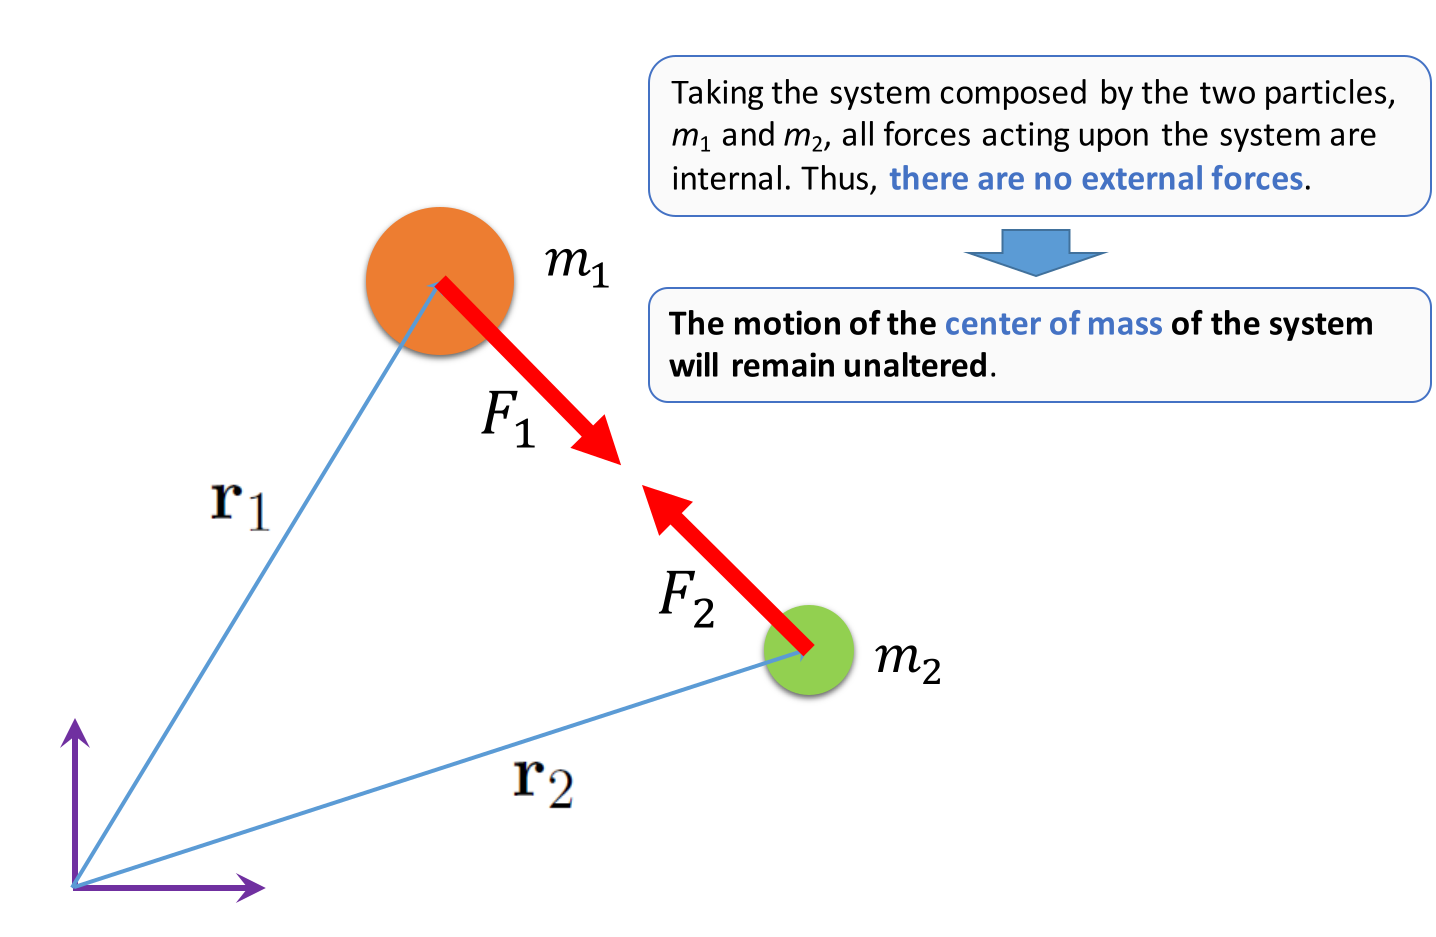
\includegraphics[width=0.75\textwidth]{Images/TBP2.png}
    \end{figure}
\end{frame}

\begin{frame}{Review: Two Body Problem}
    \begin{figure}
        \centering
        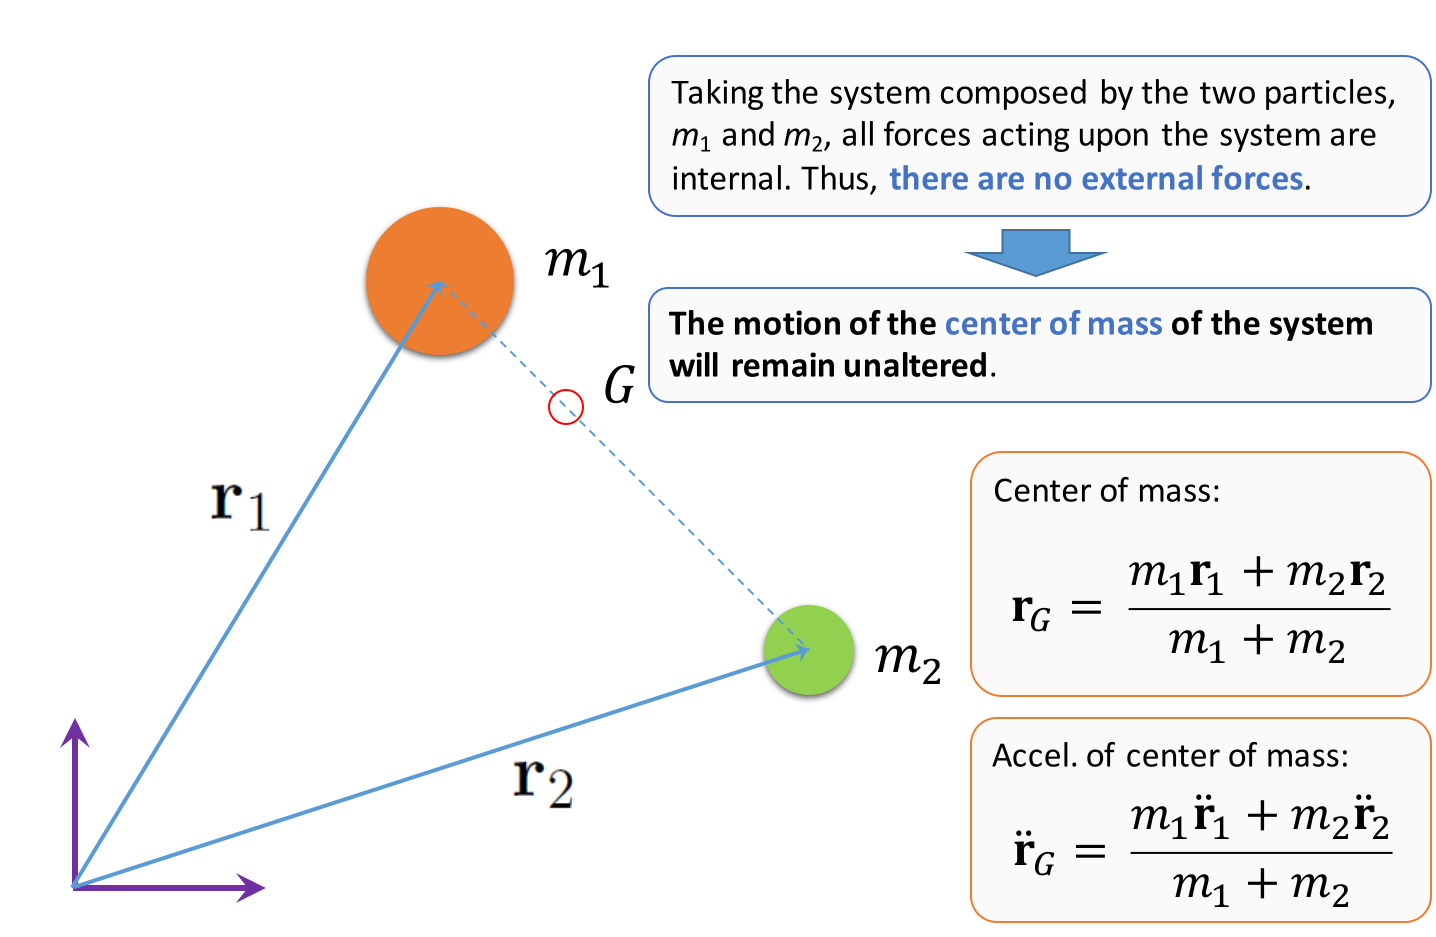
\includegraphics[width=0.75\textwidth]{Images/TBP3.png}
    \end{figure}
\end{frame}

\begin{frame}{Review: Two Body Problem}
    \begin{figure}
        \centering
        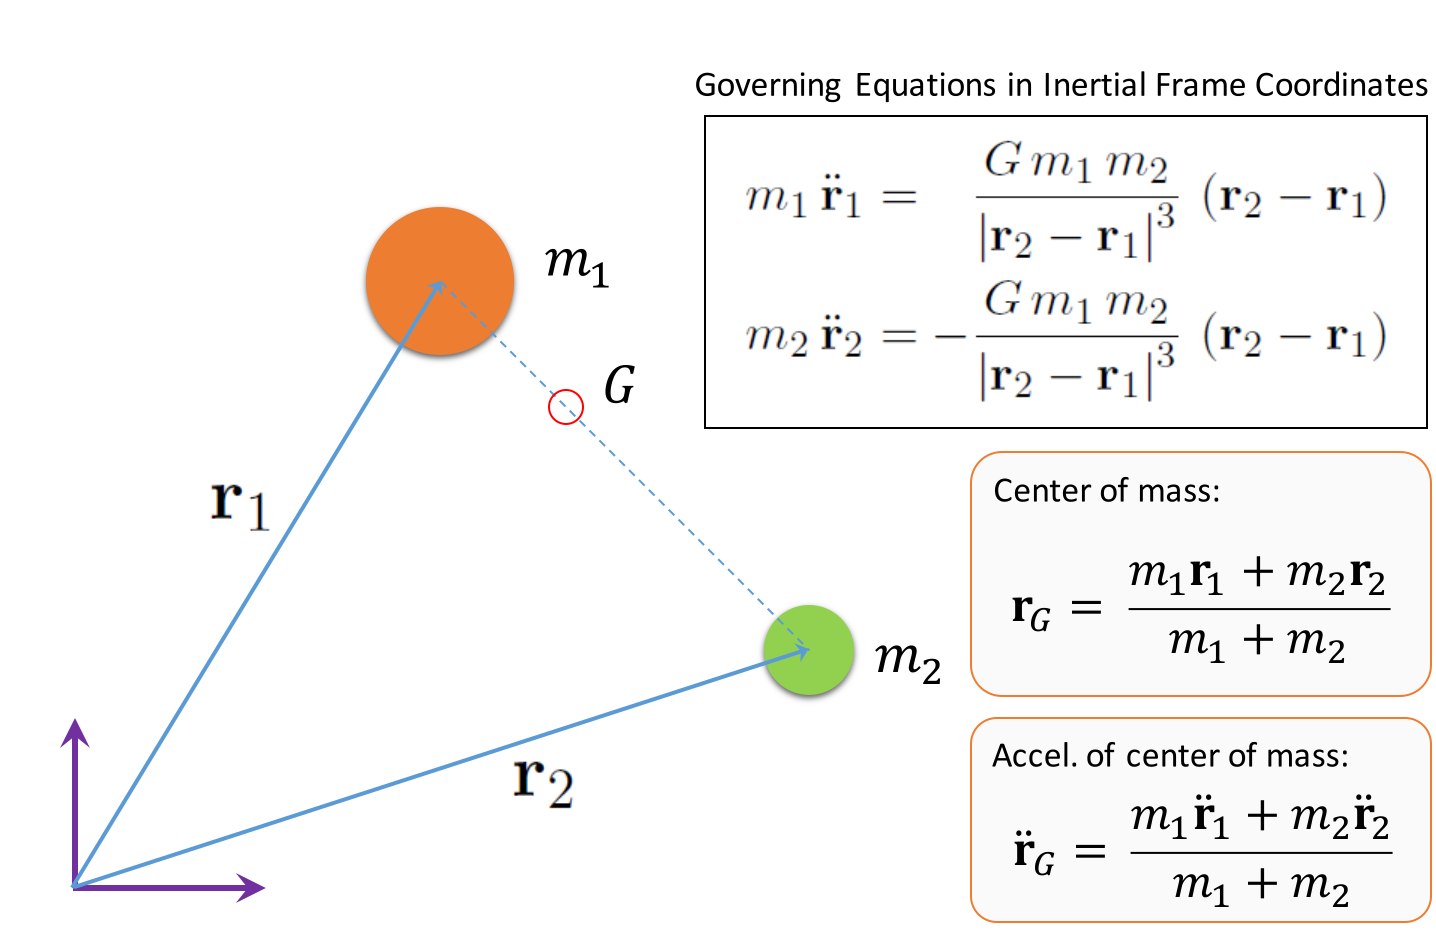
\includegraphics[width=0.75\textwidth]{Images/TBP4.png}
    \end{figure}
\end{frame}

\begin{frame}{Review: Two Body Problem}
    \begin{figure}
        \centering
        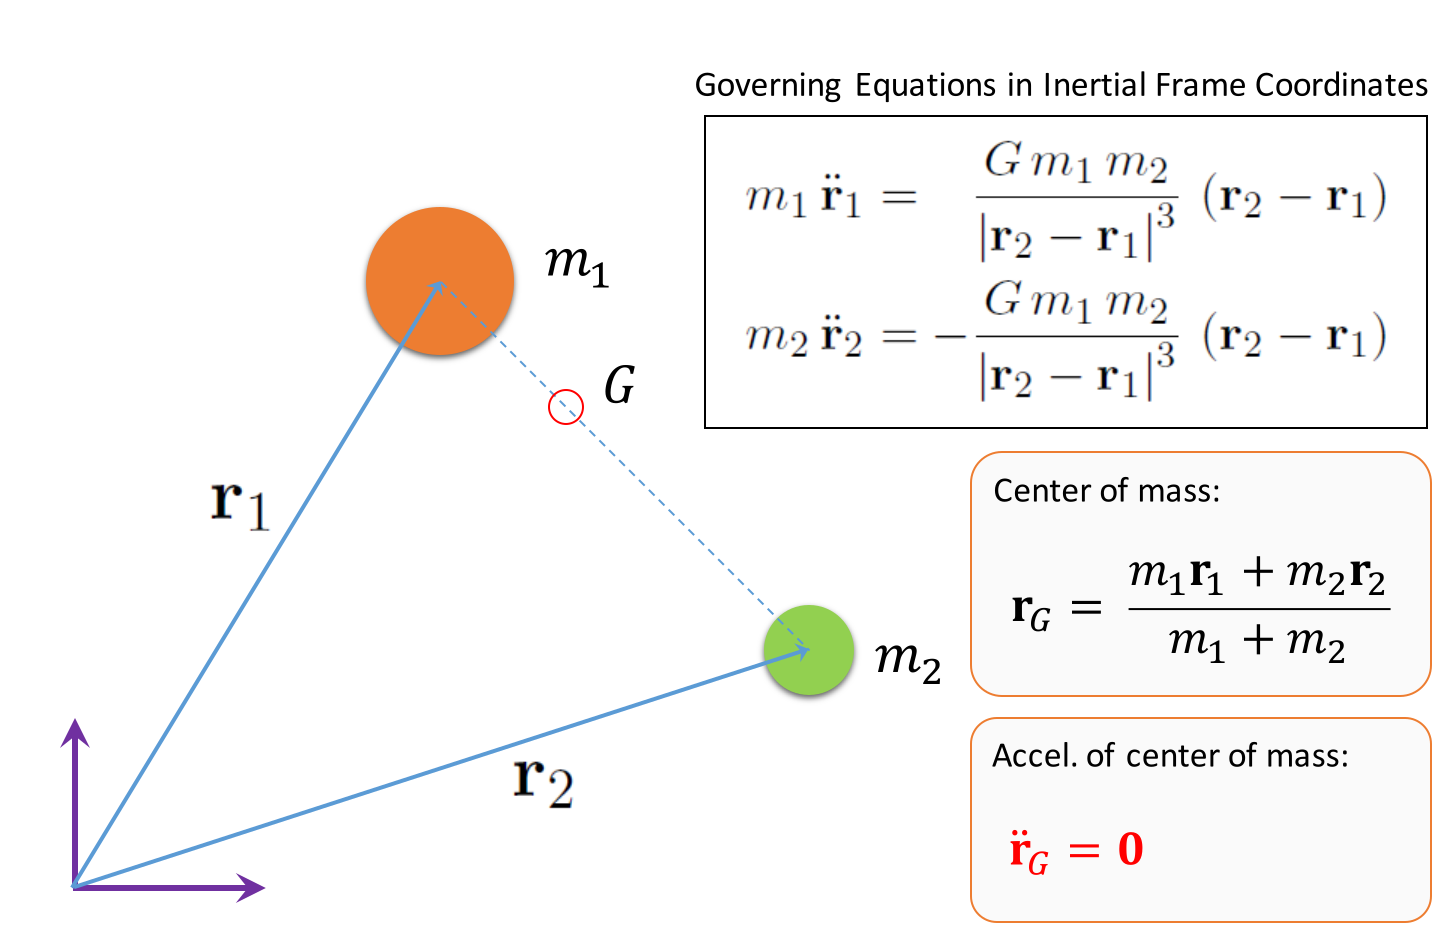
\includegraphics[width=0.75\textwidth]{Images/TBP5.png}
    \end{figure}
\end{frame}

\begin{frame}{Review: Two Body Problem}
    \begin{figure}
        \centering
        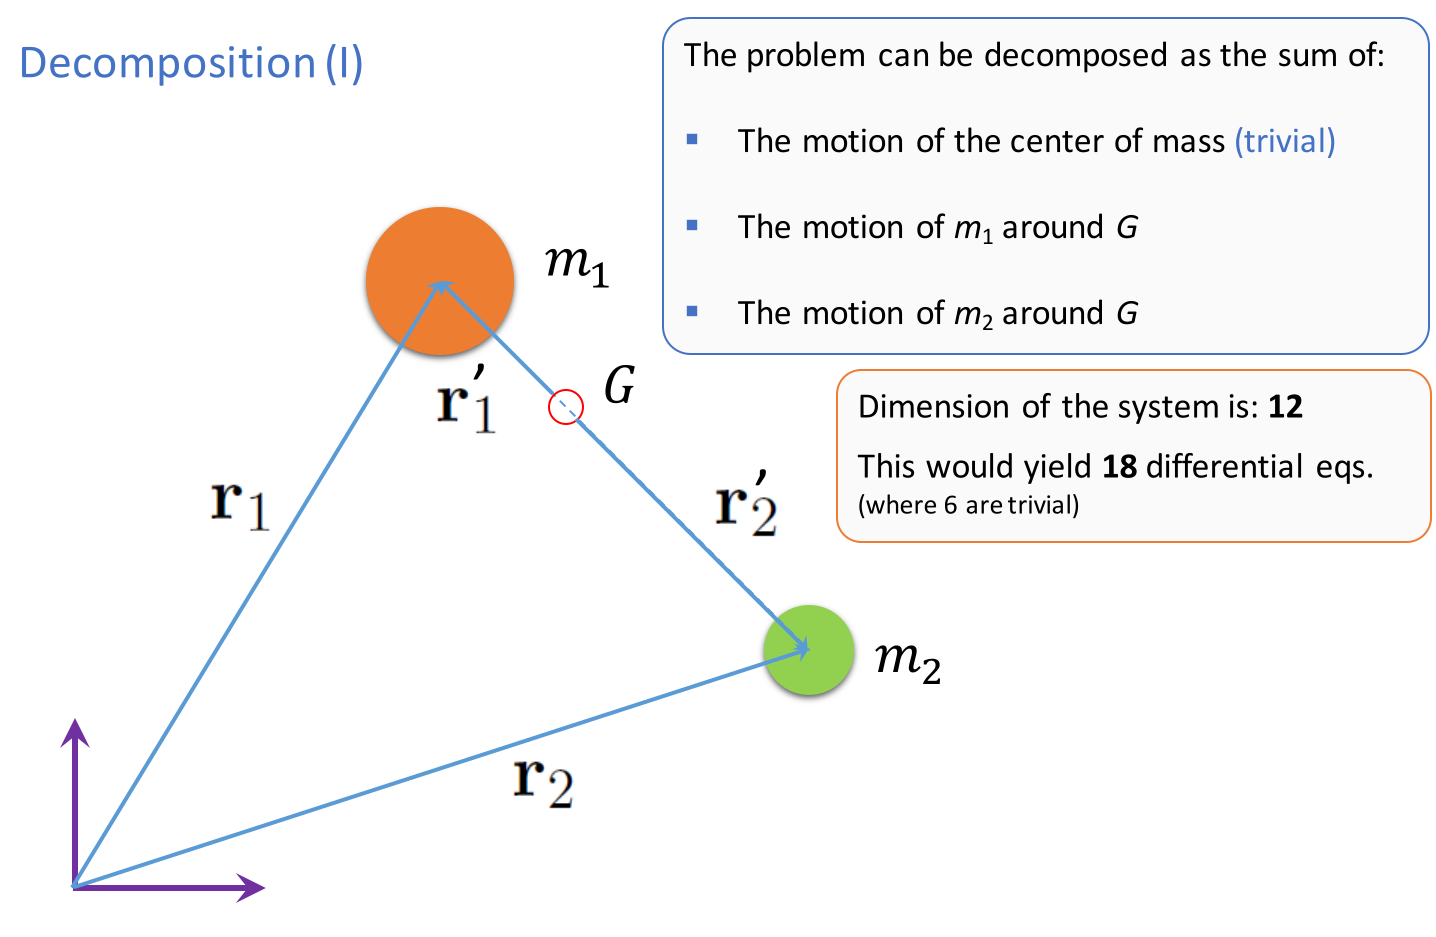
\includegraphics[width=0.75\textwidth]{Images/TBP6.png}
    \end{figure}
\end{frame}

\begin{frame}{Review: Two Body Problem}
    \begin{figure}
        \centering
        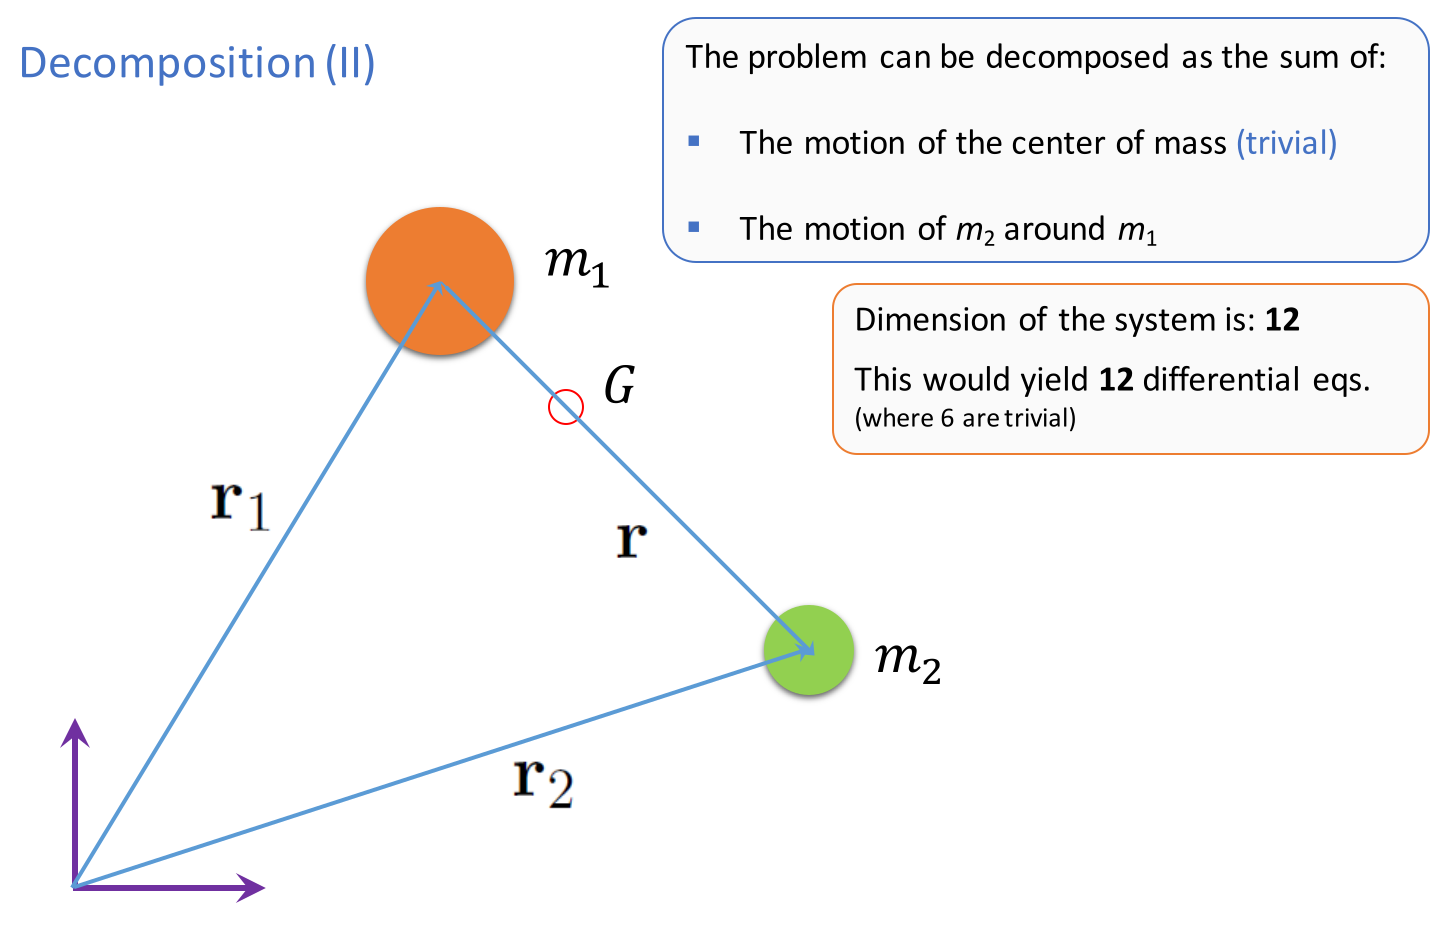
\includegraphics[width=0.75\textwidth]{Images/TBP7.png}
    \end{figure}
\end{frame}

\begin{frame}{Review: Two Body Problem}
    \begin{figure}
        \centering
        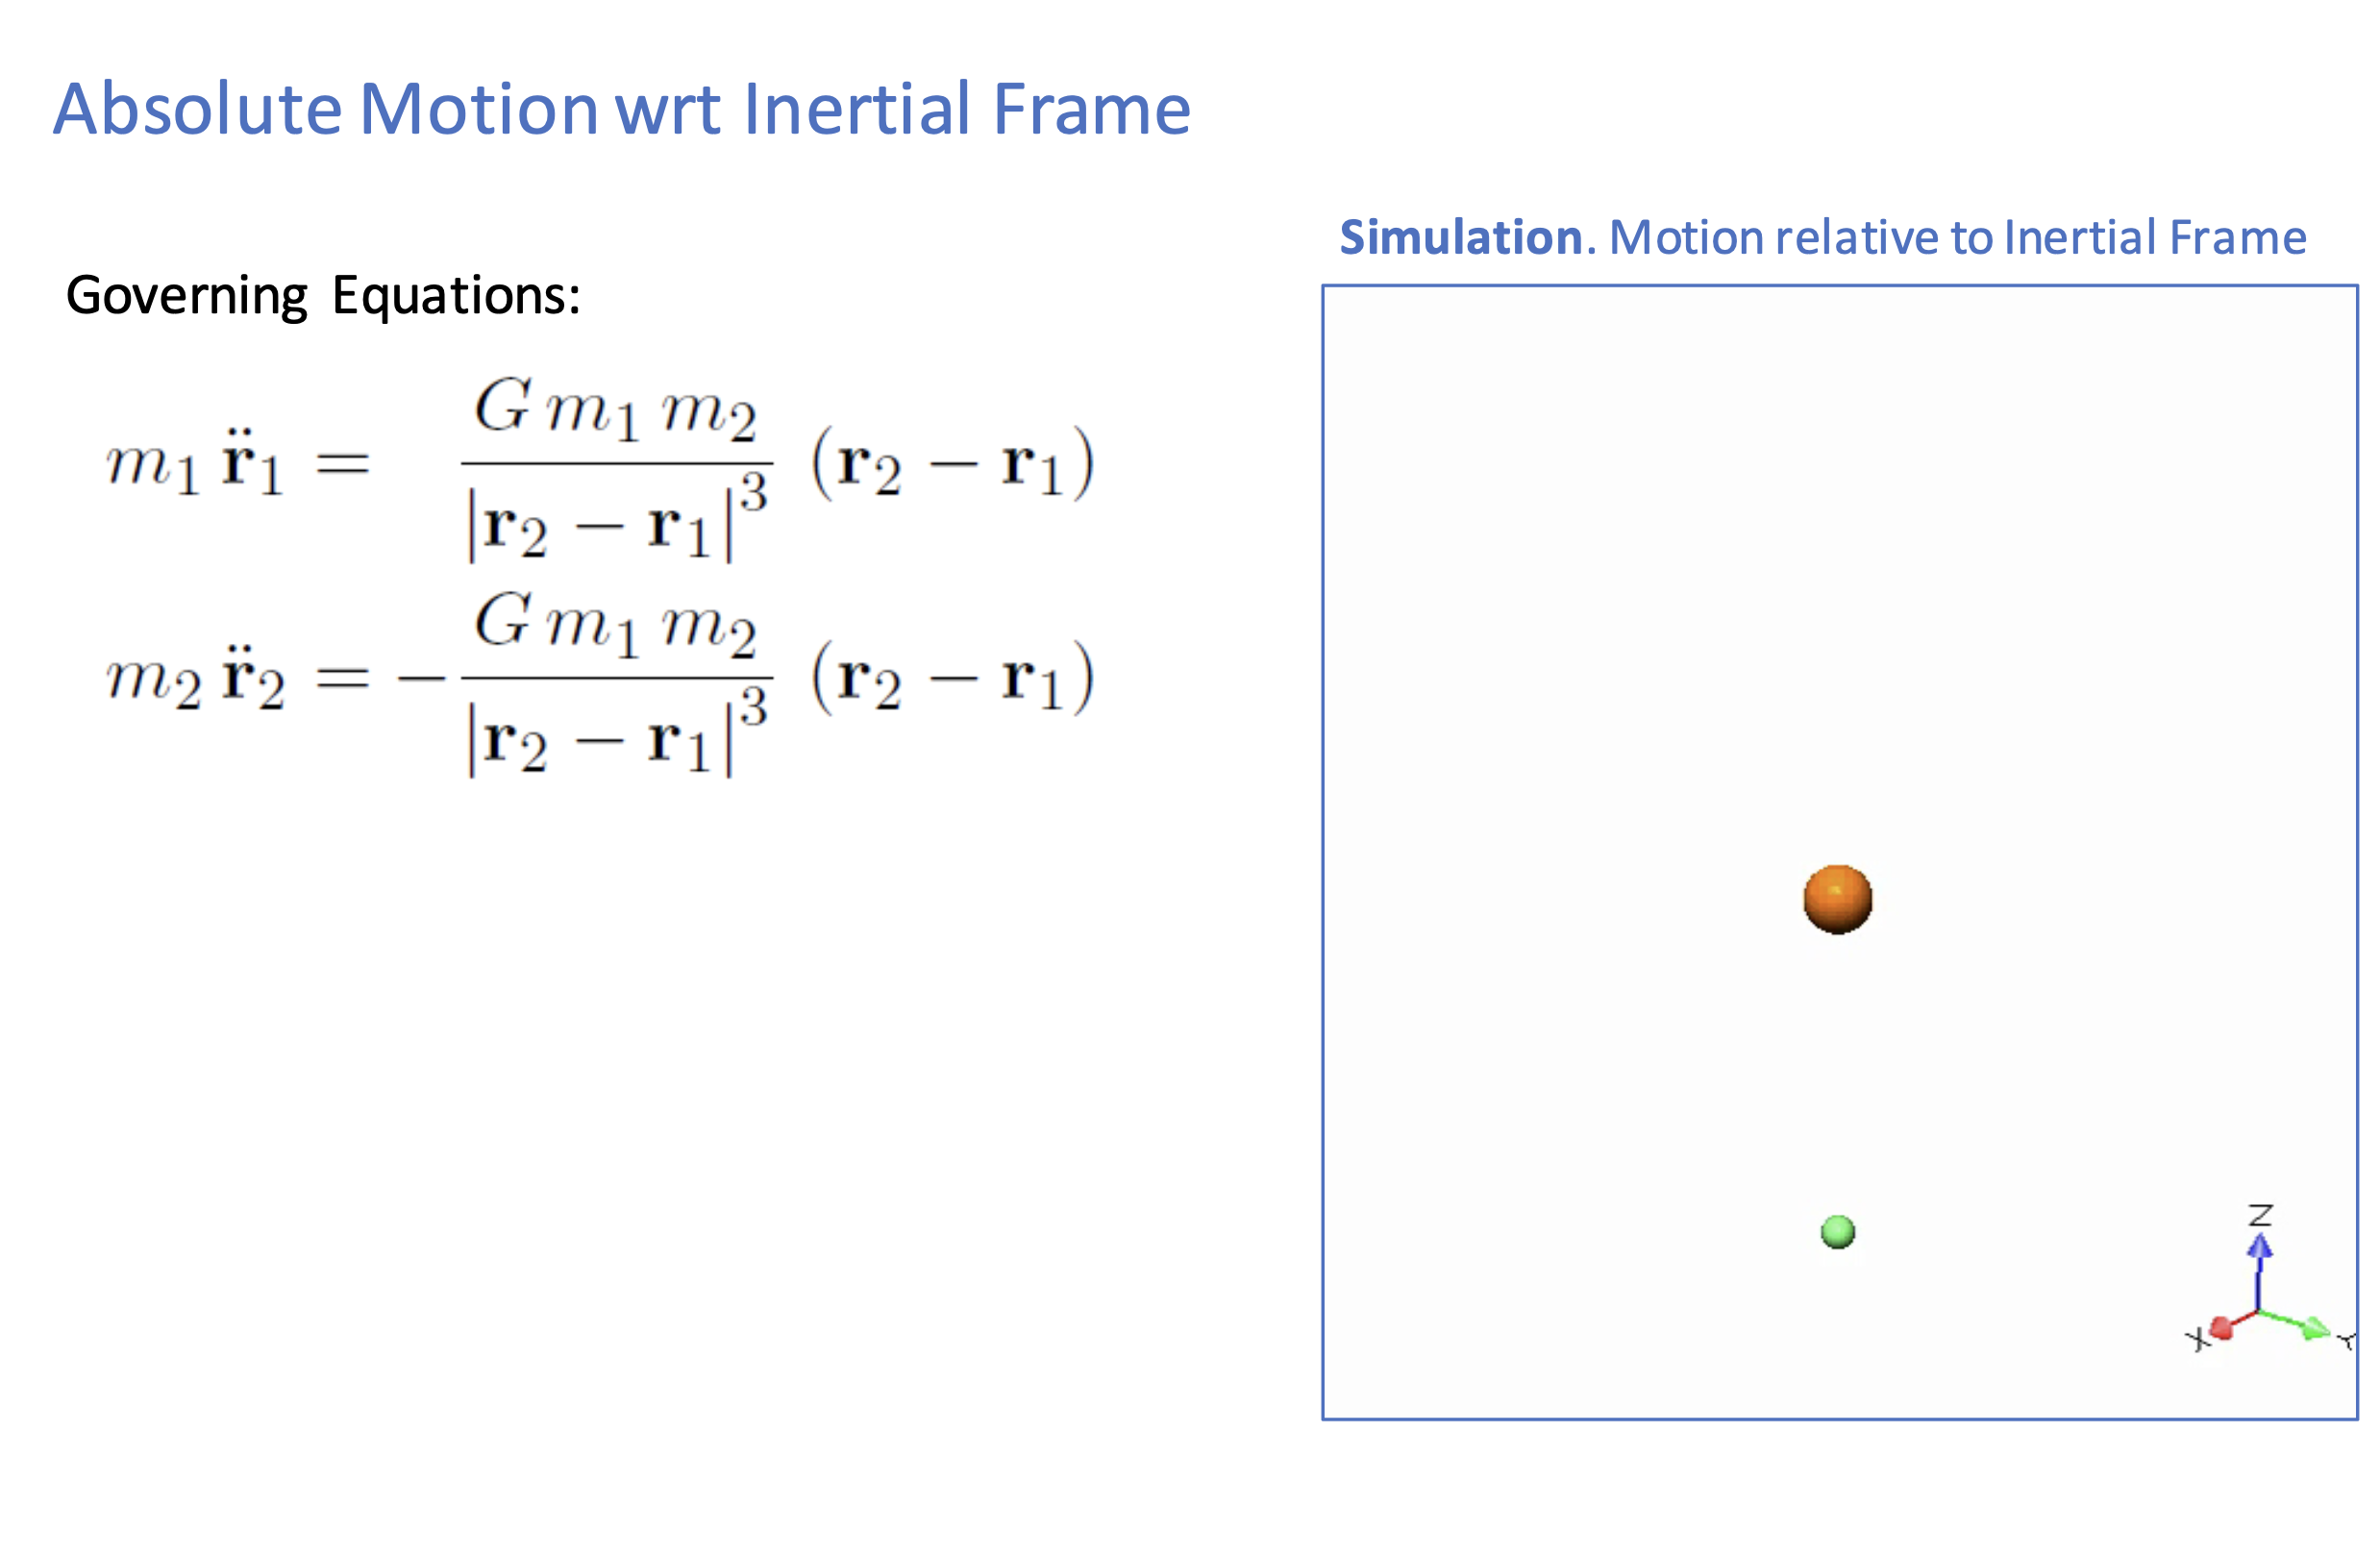
\includegraphics[width=0.75\textwidth]{Images/inertial_frame_1.png}
    \end{figure}
\end{frame}

\begin{frame}{Review: Two Body Problem}
    \begin{figure}
        \centering
        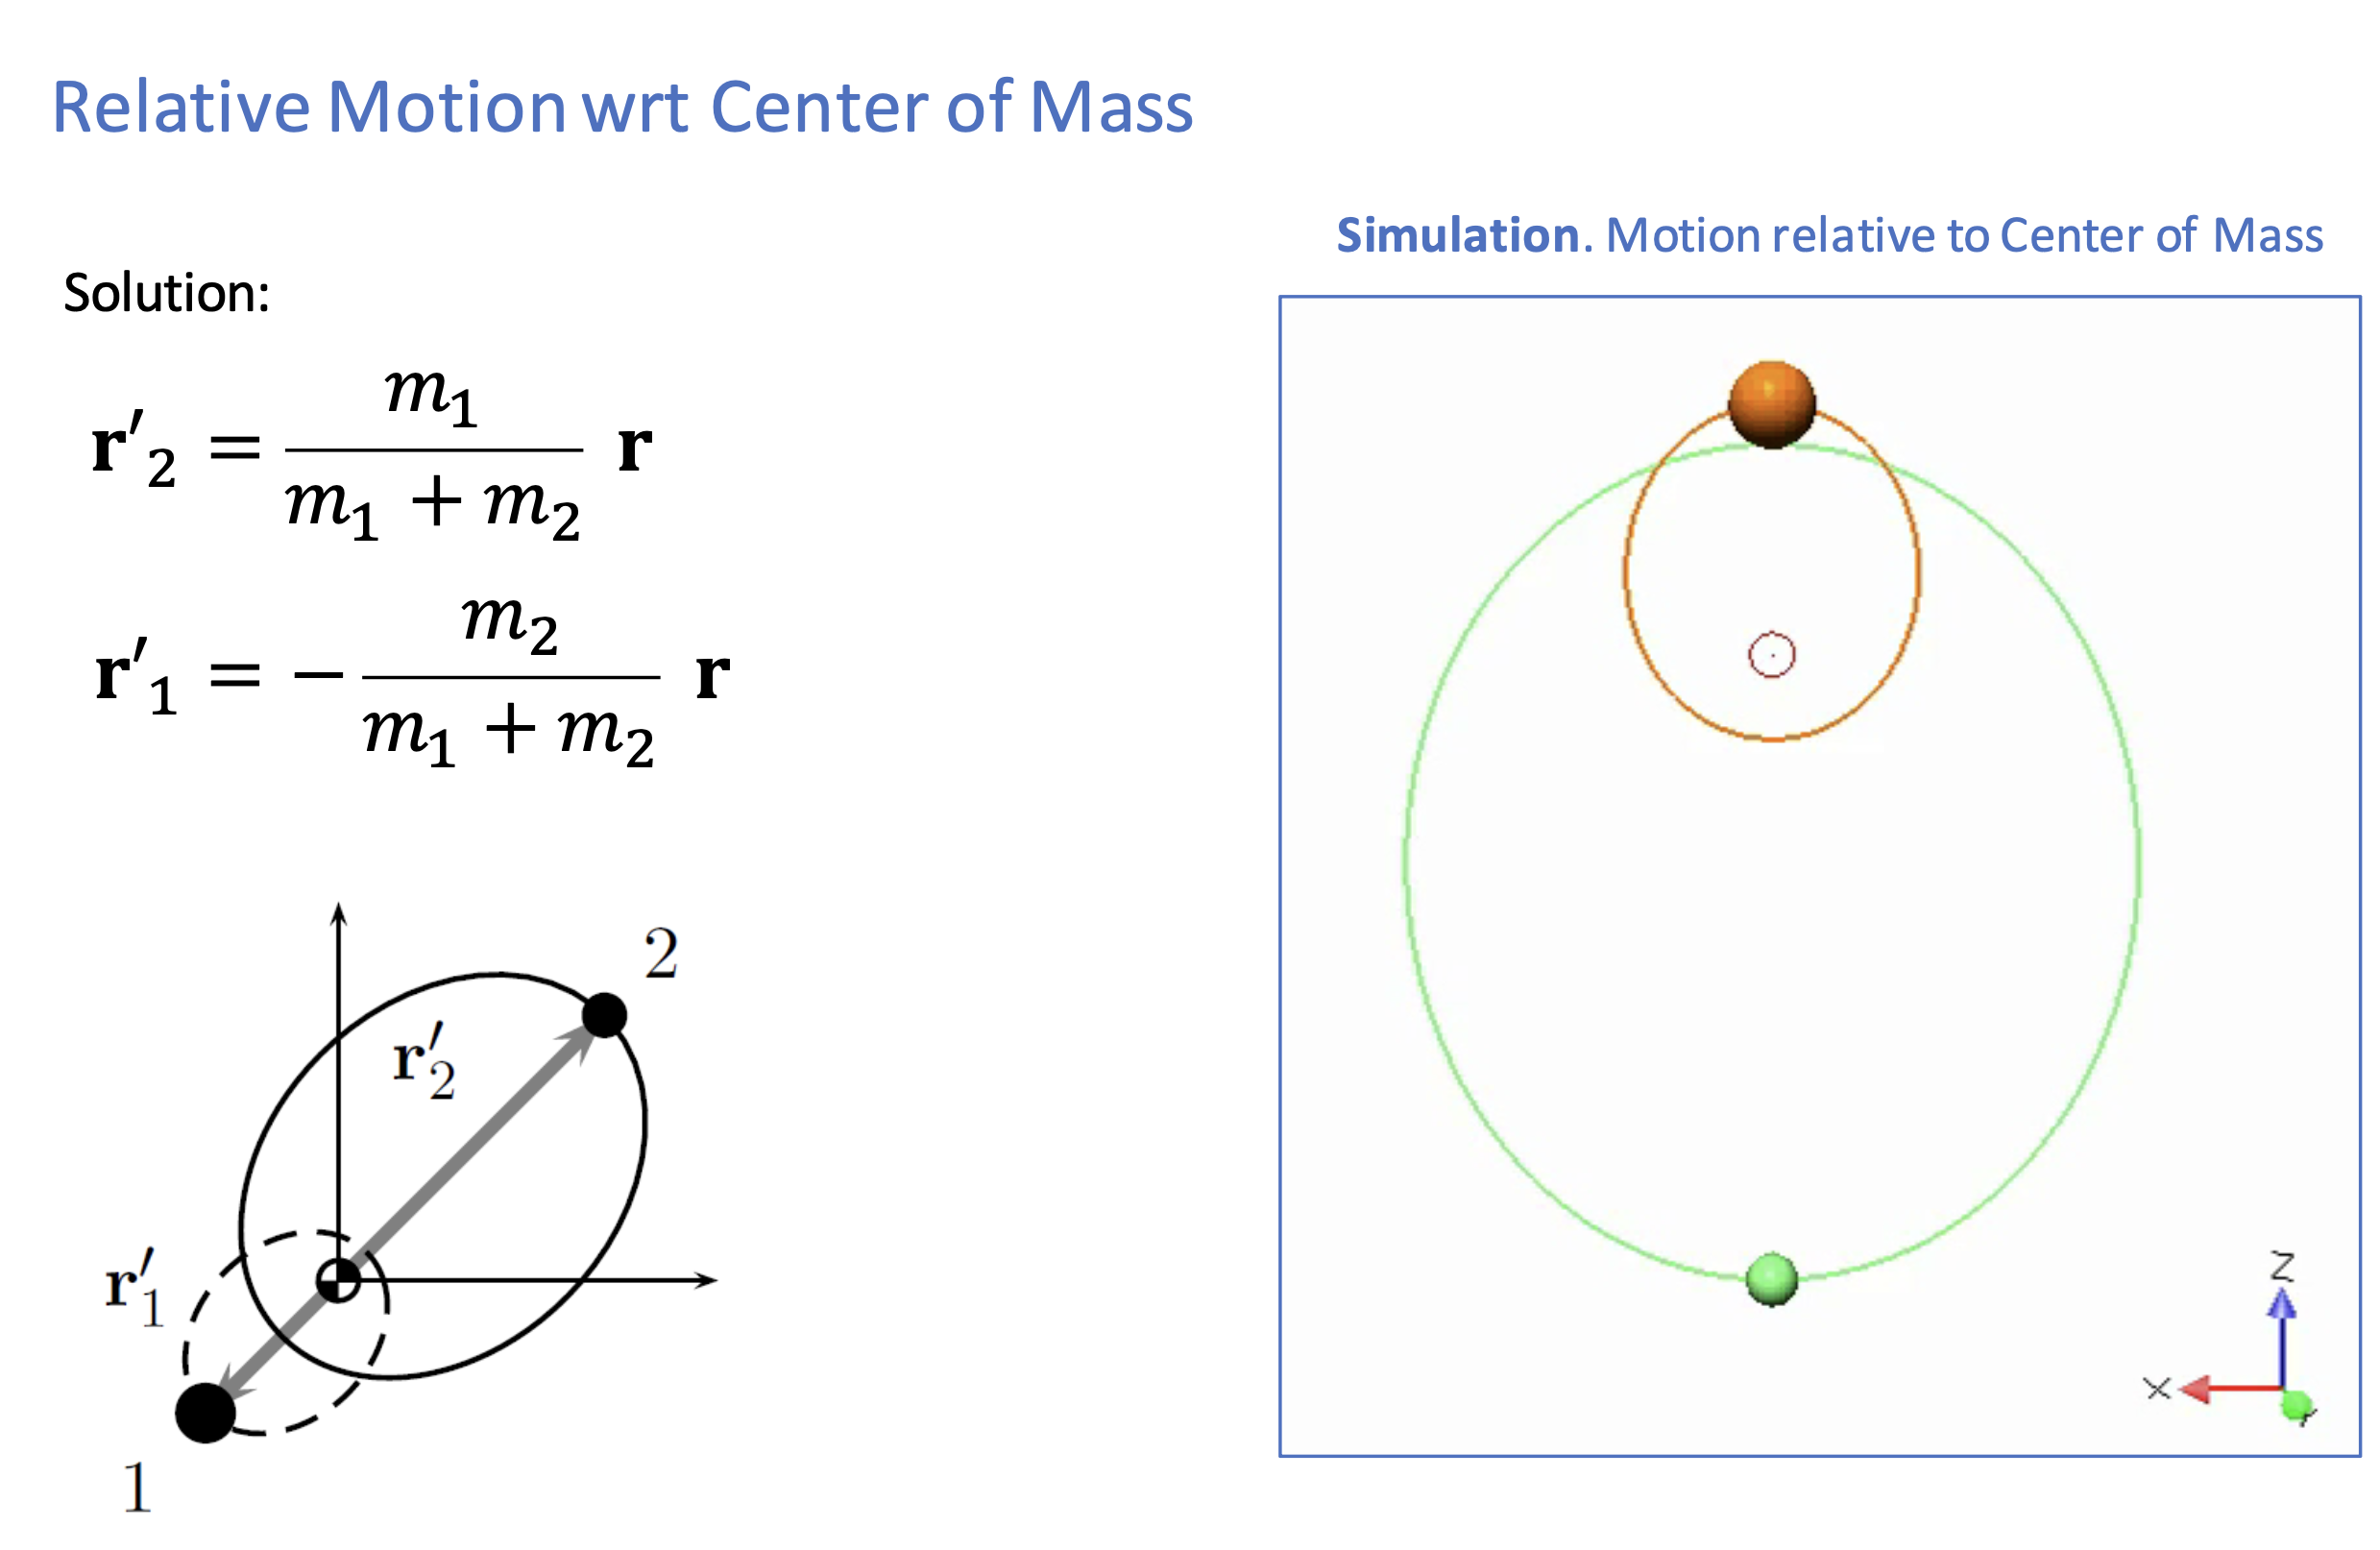
\includegraphics[width=0.75\textwidth]{Images/inertial_frame_2.png}
    \end{figure}
\end{frame}

\begin{frame}{Review: Two Body Problem}
    \begin{figure}
        \centering
        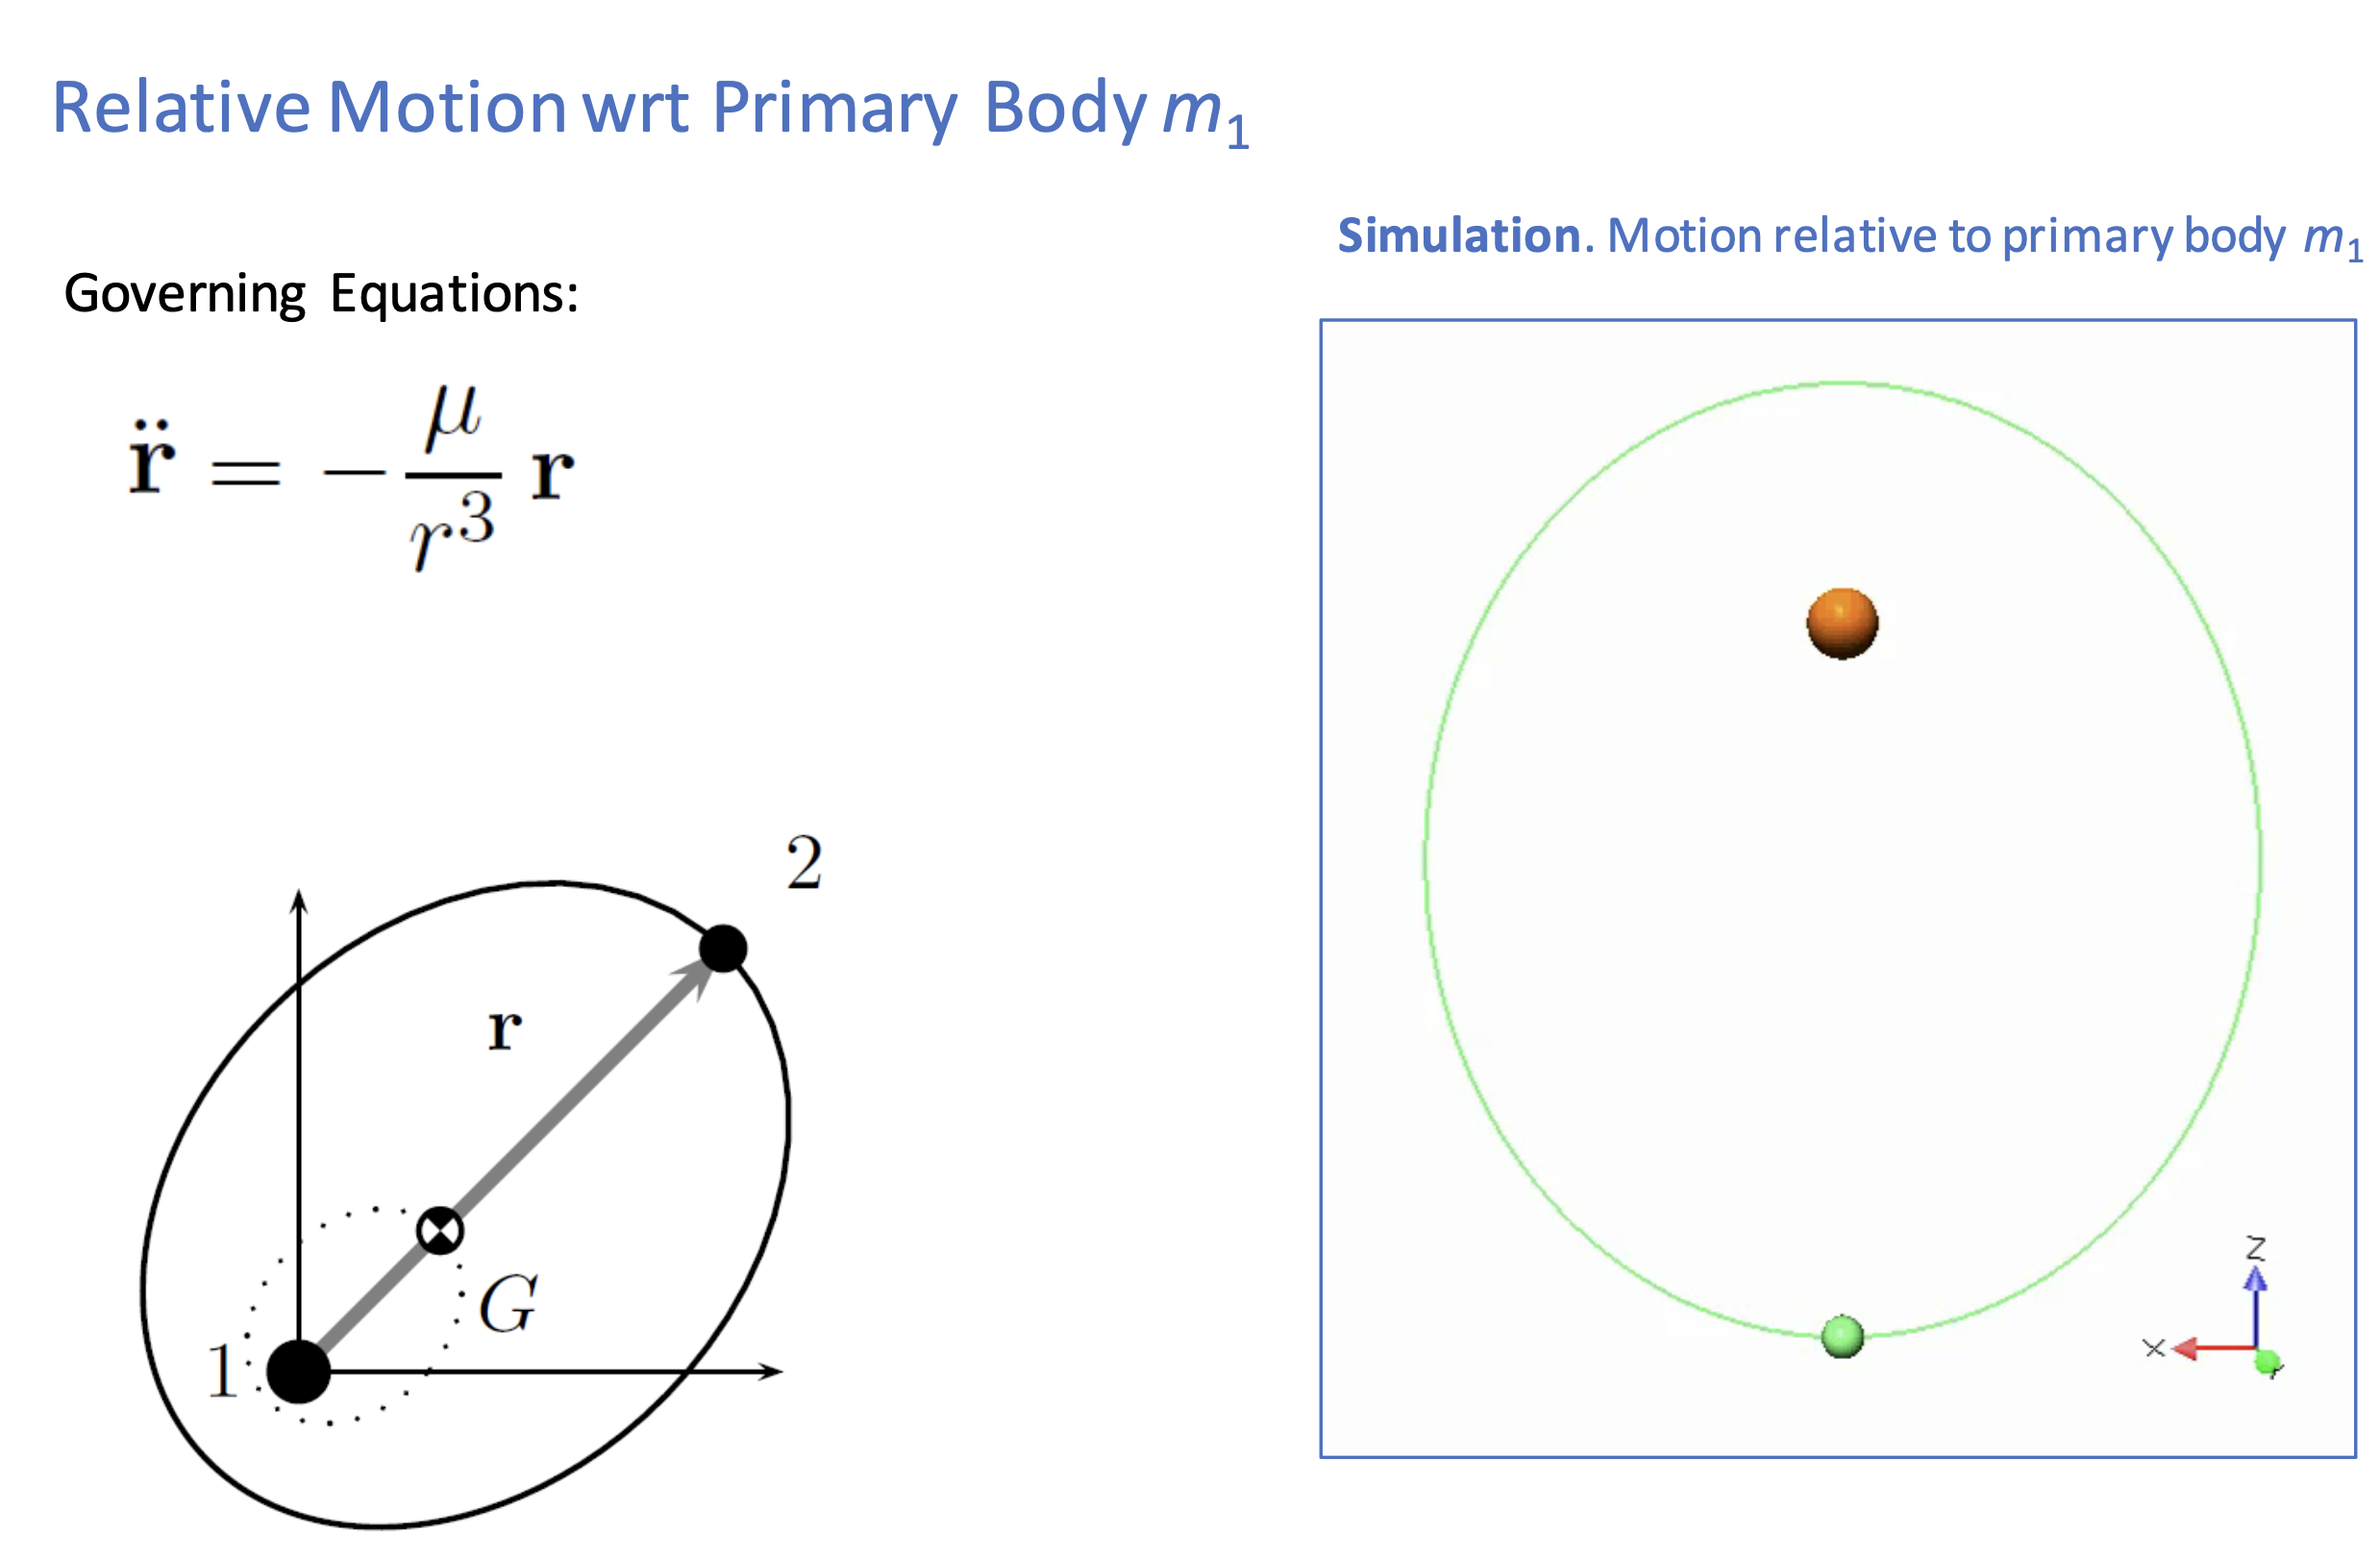
\includegraphics[width=0.75\textwidth]{Images/inertial_frame_3.png}
    \end{figure}
\end{frame}

\begin{frame}{Review: Two Body Problem}
    \begin{figure}
        \centering
        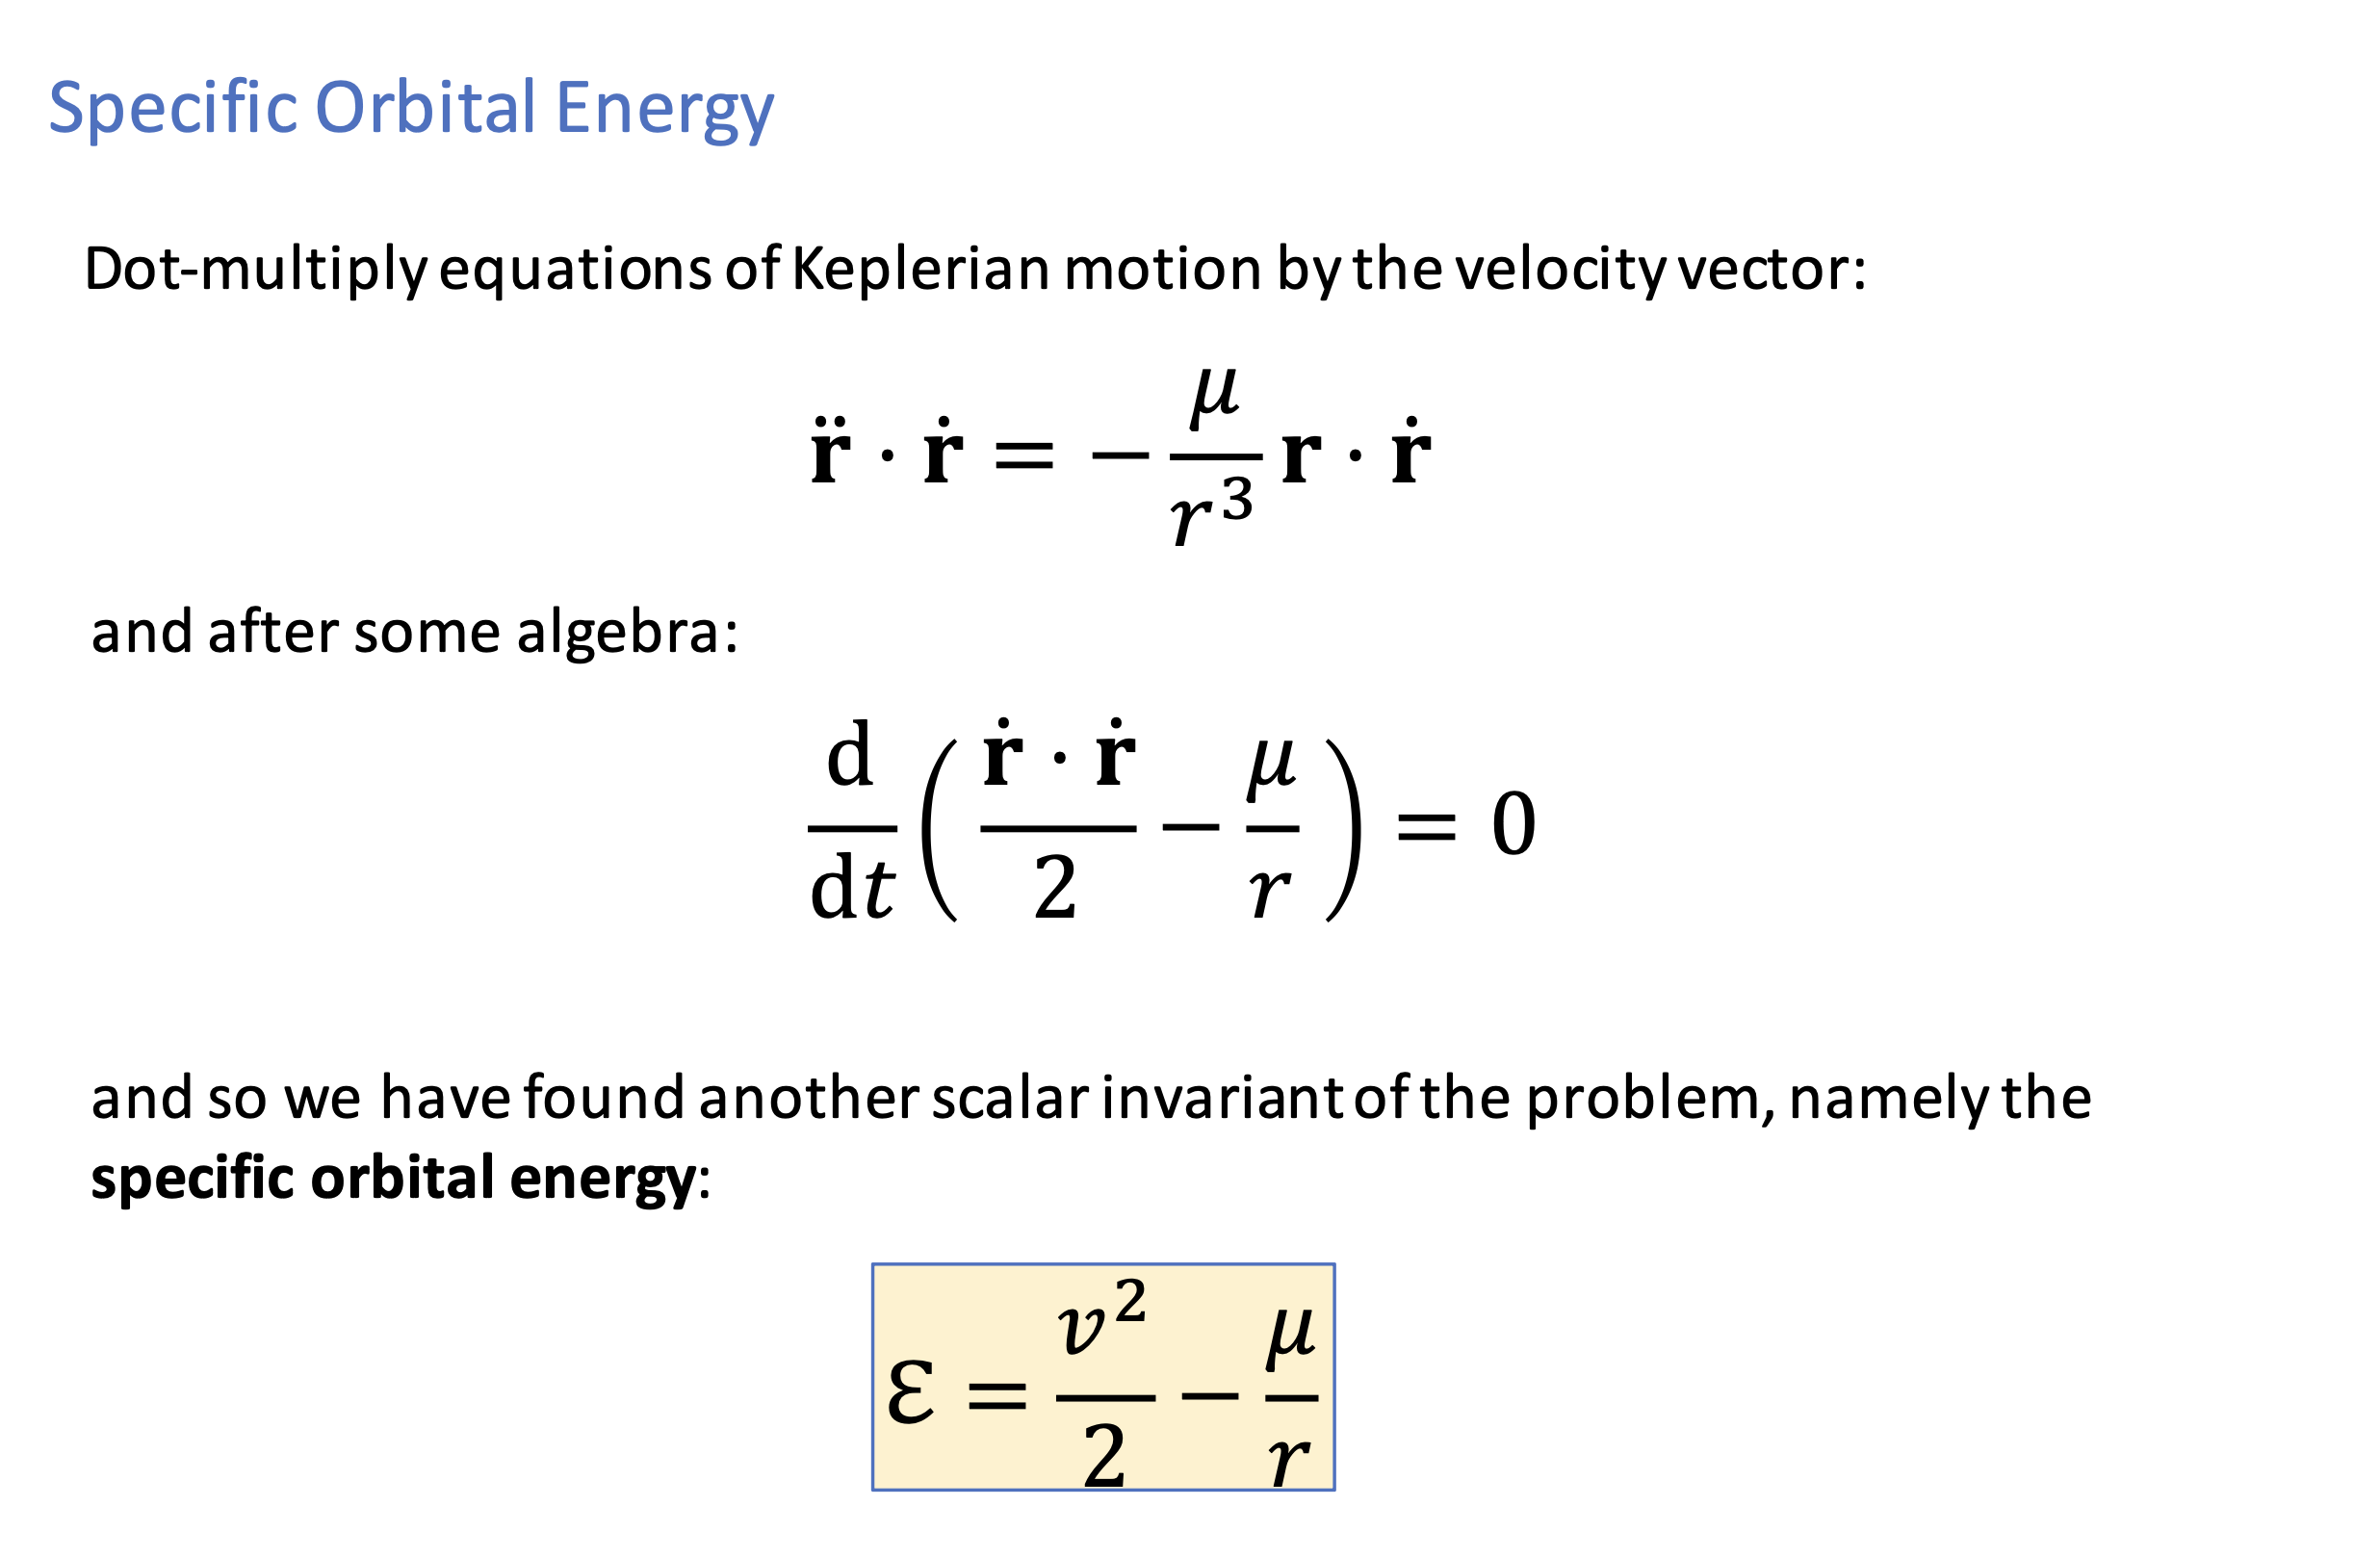
\includegraphics[width=0.75\textwidth]{Images/orbital_energy_1.png}
    \end{figure}
\end{frame}

\begin{frame}{Review: Two Body Problem}
    \begin{figure}
        \centering
        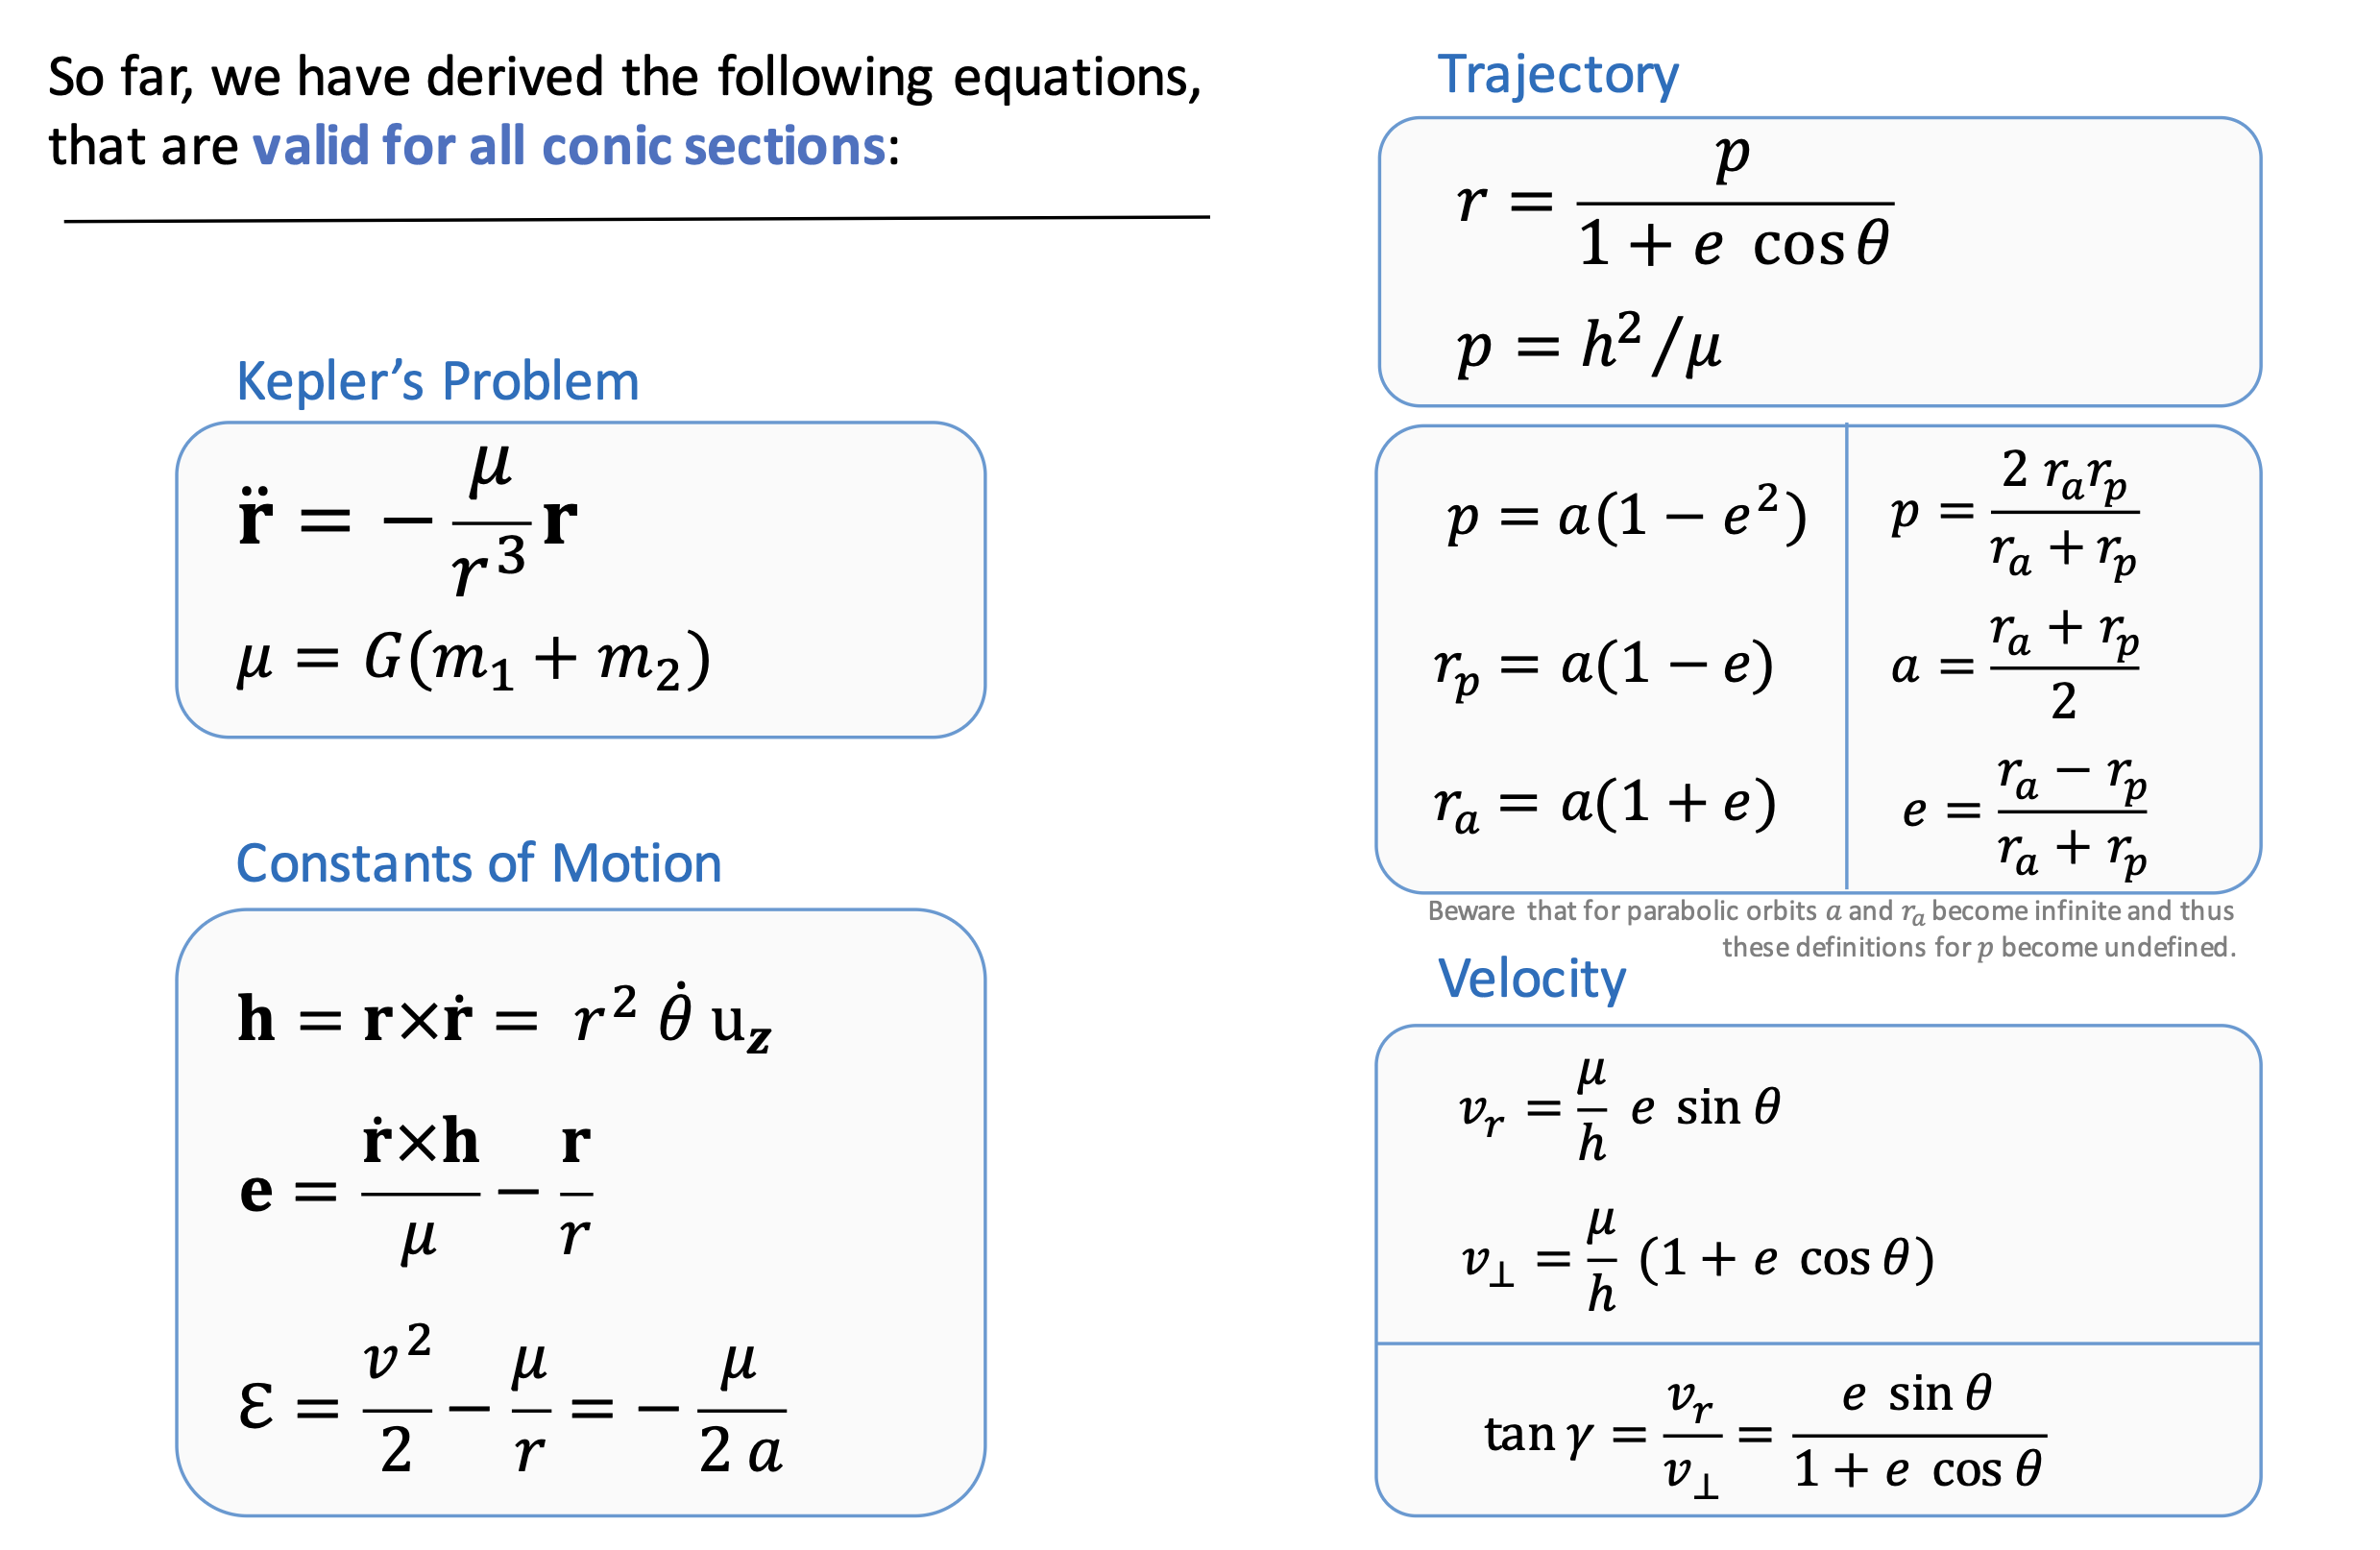
\includegraphics[width=0.75\textwidth]{Images/summary_equations.png}
    \end{figure}
\end{frame}

\begin{frame}{Review: Two Body Problem}
    \begin{figure}
        \centering
        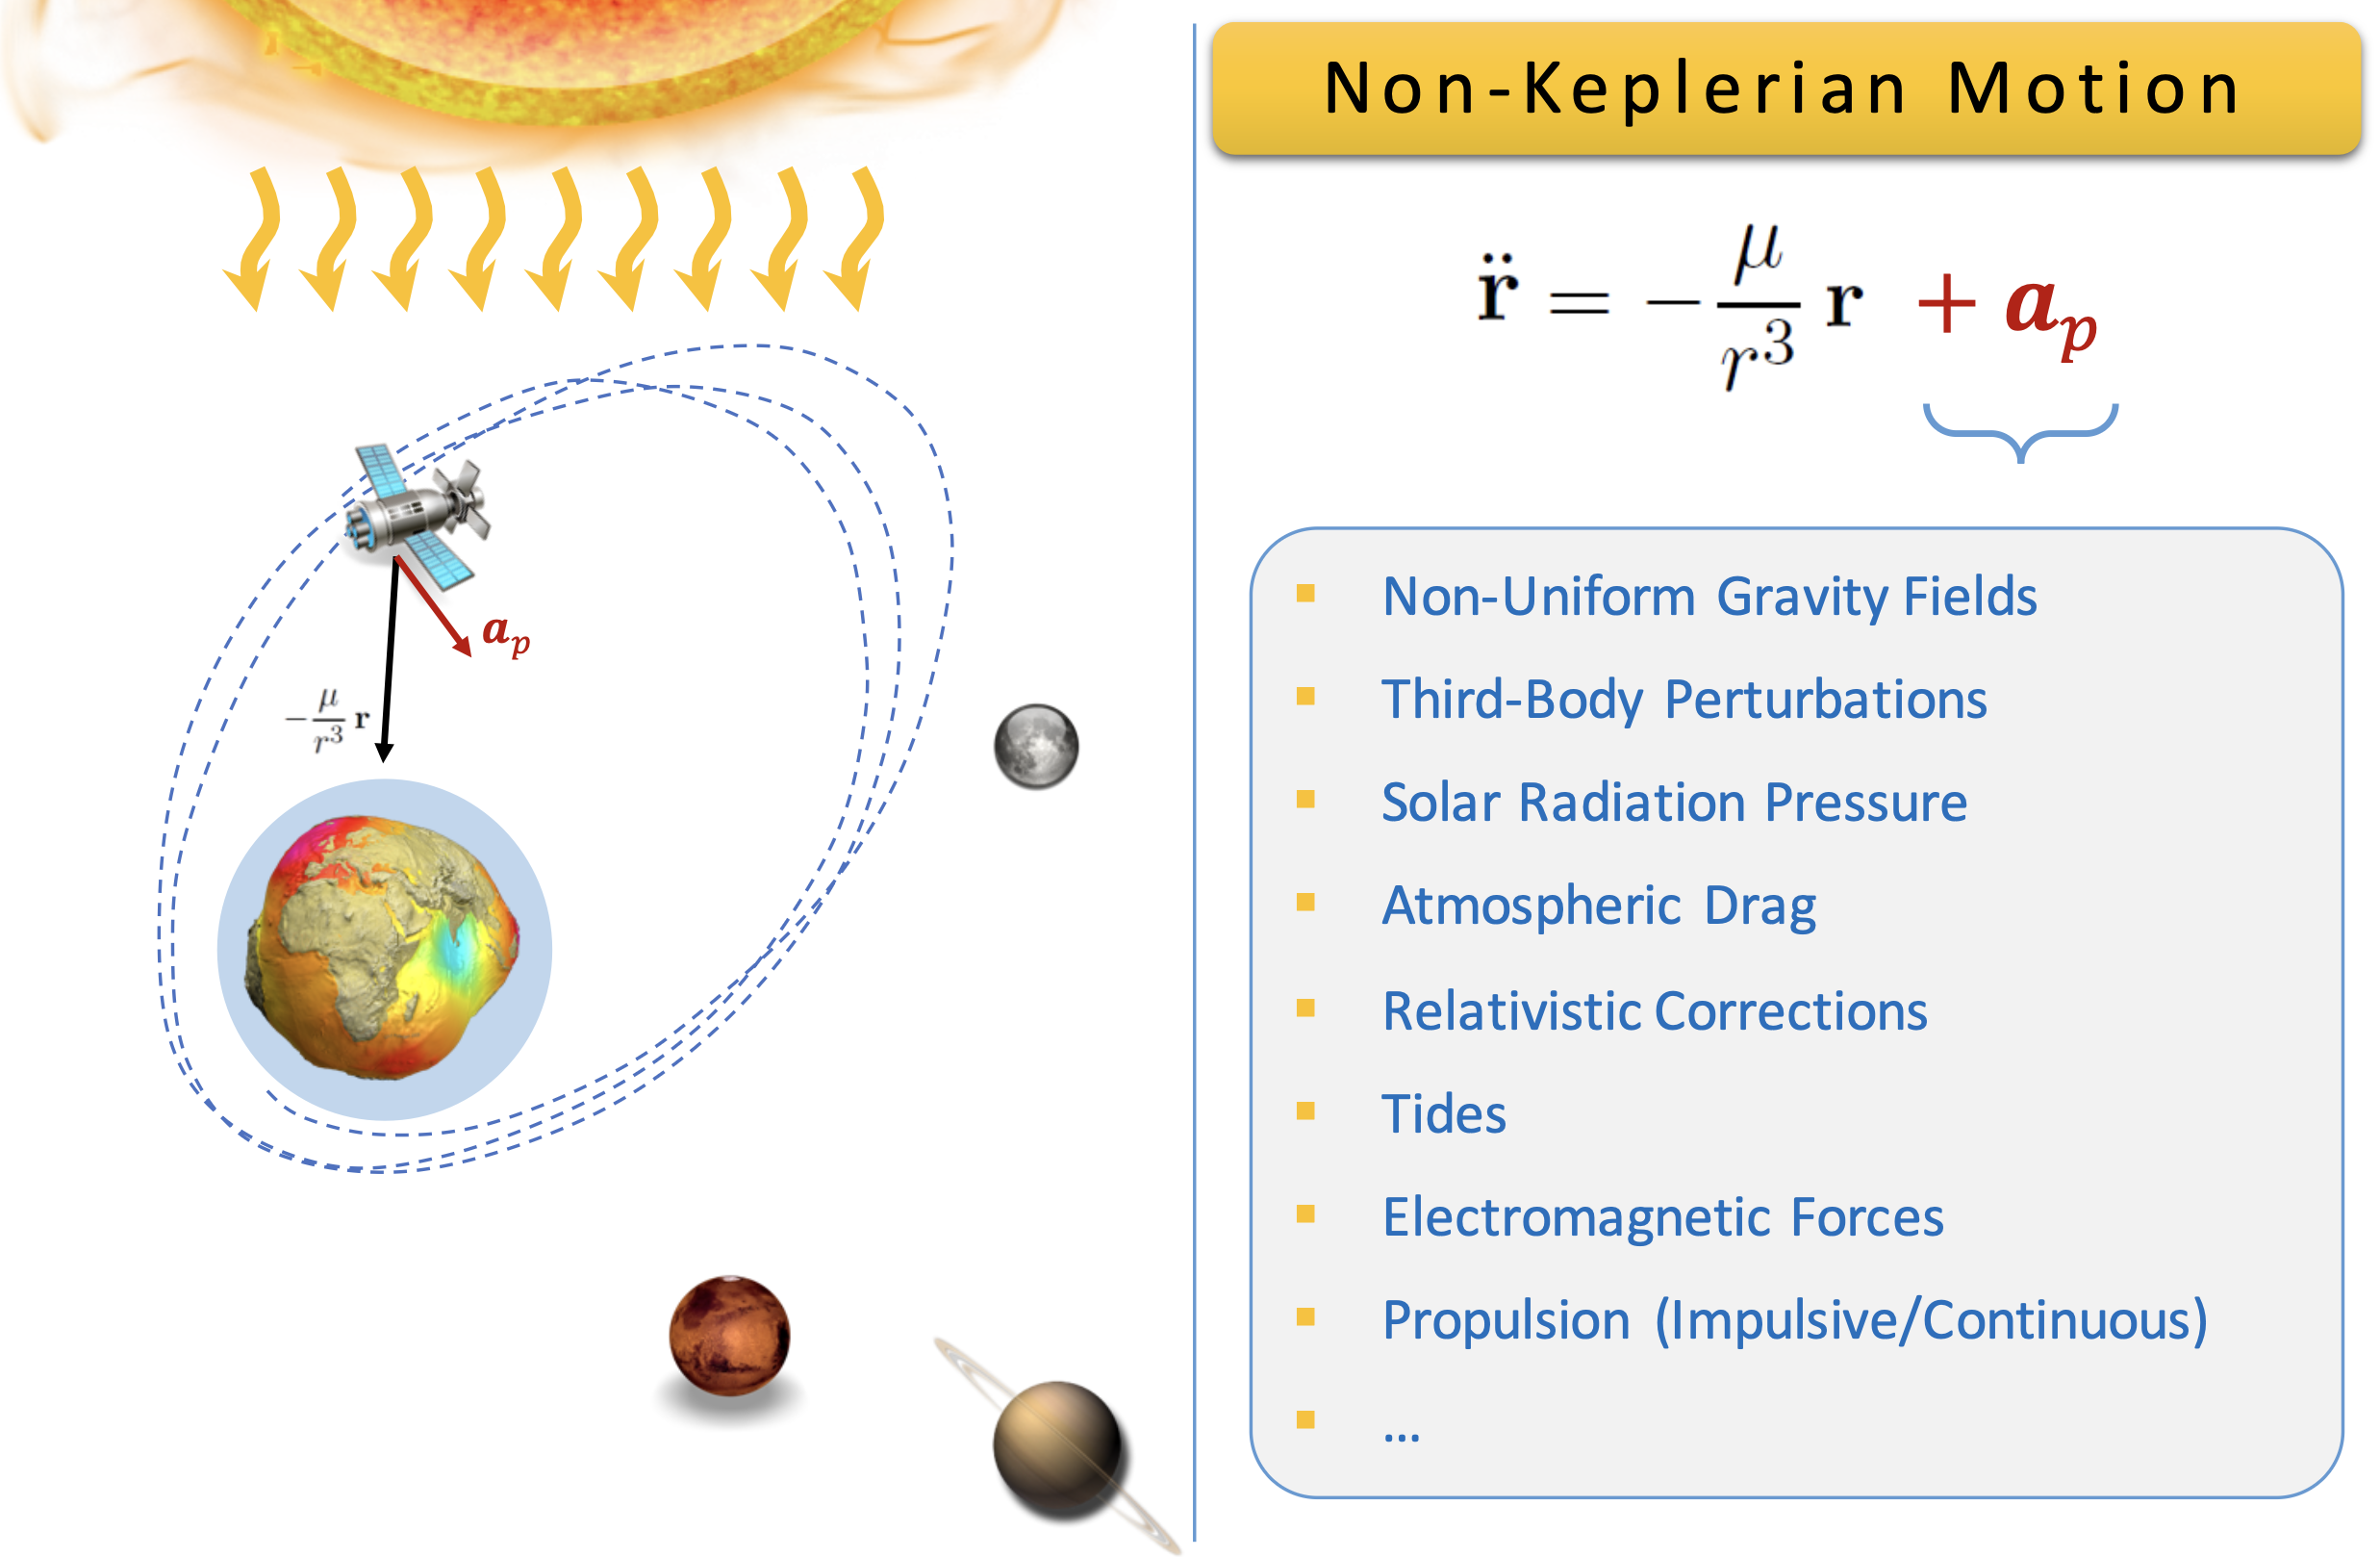
\includegraphics[width=0.75\textwidth]{Images/orbital_perturbations_1.png}
    \end{figure}
\end{frame}

\section{Introduction to Perturbed Orbits}

\begin{frame}{Real World vs. Two-Body Keplerian Motion}
    \begin{block}{Ideal Two-Body Acceleration}
        $$\mathbf{a}_{\text{Kepler}} = -\frac{\mu}{r^3}\mathbf{r}$$
        Assumes point masses, spherical symmetry, and a vacuum environment.
    \end{block}

    \vspace{0.2cm}

    \begin{block}{Perturbed Equation of Motion}
        $$\ddot{\mathbf{r}} = -\frac{\mu}{r^3}\mathbf{r} + \mathbf{a}_{\text{perturbation}}$$
        where the perturbing accelerations are modeled as:
        $$\mathbf{a}_{\text{perturbation}} = \mathbf{a}_{J_2} + \mathbf{a}_{\text{drag}} + \mathbf{a}_{\text{srp}} + \mathbf{a}_{\text{mag}} + \mathbf{a}_{3\text{rd-body}}$$
    \end{block}

    \begin{itemize}
        \item Causes orbital elements $(a, e, i, \Omega, \omega, \nu)$ to deviate from constant Keplerian conics.
        \item Divided into \textbf{gravitational} (conservative) and \textbf{non-gravitational} (dissipative/external) forces.
    \end{itemize}
\end{frame}

% ------------------------------------------------------------------------------
% SECTION 2: J2 PERTURBATION
% ------------------------------------------------------------------------------
\section{Earth Oblateness ($J_2$ Perturbation)}

\begin{frame}{Earth Oblateness ($J_2$): Physics and Potential Expansion}
    \begin{columns}
        \begin{column}{0.55\textwidth}
            \begin{itemize}
                \item Earth's diurnal rotation produces equatorial bulging ($R_e \approx 6378\text{ km}$, $R_p \approx 6356\text{ km}$).
                \item Represented via Spherical Harmonics Expansion of geopotential $V(r, \phi)$:
            \end{itemize}
            \begin{equation*}
                V(r,\phi) = -\frac{\mu}{r}\left[ 1 - \sum_{n=2}^{\infty} J_n \left(\frac{R_e}{r}\right)^n P_n(\sin\phi) \right]
            \end{equation*}
            \begin{itemize}
                \item $J_2 \approx 1.08263 \times 10^{-3}$ is $\sim 1000\times$ larger than higher zonal harmonics ($J_3, J_4$).
            \end{itemize}
        \end{column}

        \begin{column}{0.42\textwidth}
            \begin{block}{$J_2$ Acceleration}
                $$\mathbf{a}_{J_2} = \nabla V_{J_2}$$
                \begin{itemize}
                    \item Creates a non-uniform gravitational torque pulling toward the equator.
                    \item Preserves angular momentum magnitude on average, but rotates the orbital plane in space.
                \end{itemize}
            \end{block}
        \end{column}
    \end{columns}
\end{frame}

\begin{frame}{$J_2$ Secular Effects: Precession Rates}
    $J_2$ produces secular (long-term drift) changes in two primary classical orbital elements:

    \begin{block}{Nodal Precession Rate ($\dot{\Omega}$)}
        $$\dot{\Omega} = -\frac{3}{2} J_2 \left(\frac{R_e}{p}\right)^2 n \cos i \quad \text{[rad/s]}$$
        \begin{itemize}
            \item Precesses westward (retrograde) for prograde orbits ($i < 90^\circ$).
            \item Zero drift for polar orbits ($i = 90^\circ$).
        \end{itemize}
    \end{block}

    \begin{block}{Perigee Precession Rate ($\dot{\omega}$)}
        $$\dot{\omega} = \frac{3}{4} J_2 \left(\frac{R_e}{p}\right)^2 n \left( 5\cos^2 i - 1 \right) \quad \text{[rad/s]}$$
        \begin{itemize}
            \item Drift vanishes at the \textbf{critical inclination}: $i = 63.4^\circ$ or $116.6^\circ$ ($\cos^2 i = 1/5$).
        \end{itemize}
    \end{block}
\end{frame}

\begin{frame}{Engineering Applications of $J_2$}
    \begin{columns}
        \begin{column}{0.45\textwidth}
            \begin{block}{Sun-Synchronous Orbits (SSO)}
                \begin{itemize}
                    \item Target: $\dot{\Omega} = +0.9856^\circ/\text{day}$ ($360^\circ / 365.25\text{ days}$).
                    \item Matches Earth's mean orbital revolution rate around the Sun.
                    \item Ground track experiences constant local solar time illumination (ideal for optical remote sensing).
                    \item Typical LEO altitude: $\sim 600-800\text{ km}$, $i \approx 98^\circ$.
                \end{itemize}
            \end{block}
        \end{column}
        
        \begin{column}{0.45\textwidth}
            \begin{block}{Molniya Orbits}
                \begin{itemize}
                    \item Highly eccentric 12-hour period orbit ($e \approx 0.74$).
                    \item Inclination locked to $i = 63.4^\circ$.
                    \item Freezes argument of perigee ($\dot{\omega} = 0$), preventing perigee from drifting away from the Southern Hemisphere.
                    \item Maximizes dwell time over high northern latitudes.
                \end{itemize}
            \end{block}
        \end{column}
    \end{columns}
\end{frame}

% ------------------------------------------------------------------------------
% SECTION 3: ATMOSPHERIC DRAG
% ------------------------------------------------------------------------------
\section{Atmospheric Drag}

\begin{frame}{Atmospheric Drag: Physical Principles}
    \begin{block}{Drag Acceleration Model}
        $$\mathbf{a}_{\text{drag}} = -\frac{1}{2} \rho \left(\frac{C_D A}{m}\right) v_{\text{rel}} \mathbf{v}_{\text{rel}}$$
    \end{block}

    \begin{columns}
        \begin{column}{0.5\textwidth}
            \textbf{Key Parameters:}
            \begin{itemize}
                \item $\rho$: Local atmospheric density (exponential falloff with altitude).
                \item $C_D$: Drag coefficient ($\sim 2.0 - 2.2$ for complex geometries).
                \item $A/m$: Cross-sectional area-to-mass ratio [$\text{m}^2/\text{kg}$].
                \item $\mathbf{v}_{\text{rel}}$: Velocity relative to co-rotating atmosphere ($\mathbf{v} - \boldsymbol{\omega}_e \times \mathbf{r}$).
            \end{itemize}
        \end{column}

        \begin{column}{0.5\textwidth}
            \begin{block}{Ballistic Coefficient ($B^*$)}
                $$B^* = \frac{C_D A}{m}$$
                Measures vehicle susceptibility to drag. Spacecraft with large deployable arrays exhibit higher decay rates.
            \end{block}
        \end{column}
    \end{columns}
\end{frame}

\begin{frame}{Effects of Drag on Orbital Propagation}
    \begin{columns}
        \begin{column}{0.55\textwidth}
            \begin{itemize}
                \item \textbf{Energy Loss:} Dissipates total orbital mechanical energy ($E = -\mu / 2a$).
                \item \textbf{Semi-Major Axis Decay:}
                $$\frac{da}{dt} \approx -2 a^2 \frac{a_{\text{drag}}}{v} < 0$$
                \item \textbf{Orbital Circularization:} Peak drag acts at perigee (highest atmospheric density), lowering apogee much faster than perigee, driving $e \to 0$.
                \item \textbf{Paradoxical Effect:} As $a$ drops, orbital speed $v = \sqrt{\mu/a}$ actually increases!
            \end{itemize}
        \end{column}
        
        \begin{column}{0.42\textwidth}
            \begin{block}{Density Variability Drivers}
                Upper thermospheric density $\rho(h)$ varies dynamically due to:
                \begin{itemize}
                    \item 11-year Solar Activity Cycle (Extreme UV solar heating).
                    \item Geomagnetic storms.
                    \item Day/Night diurnal atmospheric bulge.
                \end{itemize}
            \end{block}
        \end{column}
    \end{columns}
\end{frame}

% ------------------------------------------------------------------------------
% SECTION 4: SOLAR RADIATION PRESSURE
% ------------------------------------------------------------------------------
\section{Solar Radiation Pressure (SRP)}

\begin{frame}{Solar Radiation Pressure (SRP): Physics}
    Photons emitted by the Sun exert momentum upon impact with satellite surfaces.

    \begin{block}{SRP Acceleration Model ("Cannonball Model")}
        $$\mathbf{a}_{\text{srp}} = - P_{\odot} C_r \left(\frac{A}{m}\right) \left(\frac{1 \text{ AU}}{r_{\odot}}\right)^2 \hat{\mathbf{u}}_{\odot}$$
    \end{block}

    \begin{columns}
        \begin{column}{0.5\textwidth}
            \textbf{Parameters:}
            \begin{itemize}
                \item $P_{\odot}$: Solar radiation constant at $1\text{ AU} \approx 4.56 \times 10^{-6}\text{ N/m}^2$.
                \item $C_r$: Radiation reflectivity ($1.0$ pure absorption, $2.0$ total specular reflection).
                \item $\hat{\mathbf{u}}_{\odot}$: Unit vector pointing toward Sun.
            \end{itemize}
        \end{column}
        
        \begin{column}{0.5\textwidth}
            \begin{block}{Eclipse / Shadow Function}
                $$\nu_{\text{shadow}} = \begin{cases} 
                    1, & \text{Direct Sunlight} \\
                    (0, 1), & \text{Penumbra} \\
                    0, & \text{Umbra (Total Shadow)}
                \end{cases}$$
                Requires tracking Earth's shadow cone geometries during orbit propagation.
            \end{block}
        \end{column}
    \end{columns}
\end{frame}

\begin{frame}{SRP Effects at High Altitudes and Solar Sailing}
    \begin{itemize}
        \item \textbf{Dominance in HEO/GEO:} While Drag dominates low LEO ($< 600\text{ km}$), SRP becomes the leading non-gravitational force in MEO, GEO, and high-altitude orbits.
        \item \textbf{Long-term Orbital Drift:} Induces periodic long-term variations in eccentricity ($e$) and inclination ($i$).
        \item \textbf{Space Debris Vulnerability:} Objects with very high $A/m$ ratios (e.g., thermal insulation fragments) experience massive SRP pertubation, leading to rapid eccentricity pumping and premature atmospheric entry.
    \end{itemize}

    \begin{exampleblock}{Propulsive Solar Sailing}
        Solar sails intentionally maximize $A/m$ ratios ($> 10\text{ m}^2/\text{kg}$) to harness $\mathbf{a}_{\text{srp}}$ for propellantless interplanetary maneuvering and orbital inclination changes.
    \end{exampleblock}
\end{frame}

% ------------------------------------------------------------------------------
% SECTION 5: GEOMAGNETIC INTERACTIONS
% ------------------------------------------------------------------------------
\section{Geomagnetic Field Interactions}

\begin{frame}{Geomagnetic Field Interaction Mechanisms}
    Earth's geomagnetic dipole field $\mathbf{B}$ interacts with spacecraft through two primary physical pathways:

    \begin{block}{1. Magnetic Disturbance Torques (Attitude Dynamics)}
        $$\boldsymbol{\tau}_{\text{mag}} = \mathbf{m}_{\text{sat}} \times \mathbf{B}$$
        \begin{itemize}
            \item $\mathbf{m}_{\text{sat}}$: Residual magnetic dipole moment of internal electronics and current loops.
            \item Primary attitude perturbation torque in LEO.
            \item Exploited purposefully using **Magnetorquers** ($\mathbf{m}_{\text{cmd}}$) for attitude control and reaction wheel desaturation.
        \end{itemize}
    \end{block}

    \begin{block}{2. Lorentz Force Acceleration (Translational Dynamics)}
        $$\mathbf{a}_{\text{Lorentz}} = \frac{q_{\text{sat}}}{m} \left( \mathbf{v}_{\text{rel}} \times \mathbf{B} \right)$$
        \begin{itemize}
            \item $q_{\text{sat}}$: Electrostatic charge acquired by spacecraft in ionospheric plasma.
            \item Utilized by **Electrodynamic Tethers (EDTs)** ($I \mathbf{L} \times \mathbf{B}$) to generate drag or boost forces without propellant consumption.
        \end{itemize}
    \end{block}
\end{frame}

% ------------------------------------------------------------------------------
% SECTION 6: COMPARATIVE ANALYSIS
% ------------------------------------------------------------------------------
\section{Comparative Hierarchy of Perturbations}

\begin{frame}{Acceleration Order of Magnitude Comparison}
    \begin{table}
        \centering
        \small
        \begin{tabular}{lccc}
            \toprule
            \textbf{Perturbation Source} & \textbf{LEO (500 km)} & \textbf{MEO (20,000 km)} & \textbf{GEO (35,786 km)} \\
            \midrule
            Central Earth Gravity ($\mu/r^2$) & $8.4 \text{ m/s}^2$ & $0.57 \text{ m/s}^2$ & $0.22 \text{ m/s}^2$ \\
            Earth $J_2$ Oblateness & $10^{-3} \text{ m/s}^2$ & $10^{-6} \text{ m/s}^2$ & $10^{-8} \text{ m/s}^2$ \\
            Atmospheric Drag & $10^{-4} - 10^{-6} \text{ m/s}^2$ & $\sim 0$ & $0$ \\
            Solar Radiation Pressure (SRP) & $10^{-7} \text{ m/s}^2$ & $10^{-7} \text{ m/s}^2$ & $10^{-7} \text{ m/s}^2$ \\
            3rd-Body Gravitational (Sun/Moon) & $10^{-7} \text{ m/s}^2$ & $10^{-5} \text{ m/s}^2$ & $10^{-5} \text{ m/s}^2$ \\
            Geomagnetic Lorentz Acceleration & $10^{-8} \text{ m/s}^2$ & $< 10^{-10} \text{ m/s}^2$ & $< 10^{-10} \text{ m/s}^2$ \\
            \bottomrule
        \end{tabular}
        \caption{Comparison of typical perturbing accelerations across regimes.}
    \end{table}
\end{frame}

% ------------------------------------------------------------------------------
% SECTION 7: SUMMARY
% ------------------------------------------------------------------------------
\begin{frame}{Summary for Orbit Determination and Estimation}
    \begin{enumerate}
        \item \textbf{$J_2$ Oblateness:} Conservative force causing nodal precession ($\dot{\Omega}$) and perigee rotation ($\dot{\omega}$). Basis of SSO and Molniya orbits.
        \item \textbf{Atmospheric Drag:} Non-conservative force driving semi-major axis decay ($a\downarrow$) and circularization ($e\downarrow$). Dominant perturbation in LEO.
        \item \textbf{Solar Radiation Pressure:} Non-conservative force dominating in GEO/HEO. Induces long-term eccentricity oscillations.
        \item \textbf{Geomagnetic Interactions:} Produces primary disturbance torque for attitude control; can be leveraged via magnetorquers or electrodynamic tethers.
        \item \textbf{Estimation Implications:} Precise Orbit Determination (POD) filters (EKF/Batch) must estimate dynamic atmospheric scaling factors ($B^*$) and solar reflectivity coefficients ($C_r$) alongside spacecraft position and velocity states.
    \end{enumerate}
\end{frame}

\section{Trajectory Optimization and Control}

\begin{frame}{Trajectory Optimization: Introduction}
    \begin{block}{From Impulsive to Continuous Thrust}
        Traditional orbital maneuvers assume instantaneous velocity changes ($\Delta V$). Advanced mission design, however, requires modeling continuous steering histories.
    \end{block}
    
    \vspace{0.3cm}
    \begin{itemize}
        \item \textbf{Steering History:} We move beyond a single burn vector; we define a continuous time-history of pitch $\alpha(t)$ and yaw $\beta(t)$.
        \item \textbf{The Mathematical Engine:} We utilize \textit{Optimal Control Theory}, specifically solving for the state-costate trajectories.
        \item \textbf{Numerical Discretization:} Since these problems are generally non-linear and non-analytical, we use \textbf{Collocation} to discretize the continuous path into a grid of nodes, allowing solvers to converge on an optimal steering profile.
    \end{itemize}
\end{frame}

\begin{frame}{Mathematical Foundations of Optimization}
    The goal is to minimize a cost function $J$ (e.g., fuel mass, time) subject to dynamic constraints:
    
    \[ J = \Phi(\mathbf{x}(t_f), t_f) + \int_{t_0}^{t_f} L(\mathbf{x}, \mathbf{u}, t) \, dt \]
    
    \begin{itemize}
        \item \textbf{Hamiltonians ($H$):} We incorporate Lagrange multipliers ($\lambda$) to account for mission constraints (boundary values).
        \item \textbf{Collocation Methods:} We solve the problem by satisfying differential equations at specific "nodes" along the trajectory, turning an infinite-dimensional problem into a large-scale nonlinear programming (NLP) problem.
    \end{itemize}
    
    \textit{Note: The objective is to understand the physics the math is achieving, not to perform Hamiltonian integration by hand.}
\end{frame}

\begin{frame}{Practical Lab: The Optimizer Transition}
    \begin{exampleblock}{Today's Mission: The Optimizer Audit}
        Transitioning from a blind targeter to a gradient-based optimizer (e.g., Yukon, SNOPT).
    \end{exampleblock}
    
    \begin{enumerate}
        \item \textbf{The Baseline:} Initialize a standard inclination change using a simple Differential Corrector (DC). Observe the convergence sensitivity to the initial guess.
        \item \textbf{The Upgrade:} Implement a gradient-search algorithm.
        \item \textbf{Optimization Parameters:}
        \begin{itemize}
            \item \textbf{Objective Function:} Minimize Total Burn Duration.
            \item \textbf{Path Constraint:} Maintain eccentricity $< 0.001$.
        \end{itemize}
        \item \textbf{Forensic Debrief:} Map how the optimizer traverses the parameter space compared to the targeter.
    \end{enumerate}
\end{frame}

\begin{frame}{Synthesis and Industry Best Practices}
    \begin{itemize}
        \item \textbf{Why it Matters:} Missions like \textit{Dawn} (ion propulsion) or \textit{Artemis Gateway} (NRHO transfers) rely entirely on numerical optimization—analytical math alone cannot map the solution space.
        \item \textbf{The Role of the Engineer:} Optimizers are not "magic." They require a physically sensible initial guess. If the guess is poor, the optimizer will diverge.
        \item \textbf{Industry Standard:} Engineers do not write their own solvers for deep space; they rely on established suites like GMAT (with CSALT), STK, or Copernicus. Your task is to audit the solution's validity.
    \end{itemize}
\end{frame}

\section{Week 1: Non-Keplerian Spaces and Variational Systems}

% --- WEEK 1: SLIDE 1 ---
\begin{frame}{Week 1: Moving Beyond the Two-Body Idealization}
    The exact differential vector equation of motion for a point mass under conservative, non-spherical, and non-conservative forces is given by:
    \[ \ddot{\mathbf{r}} = -\frac{\mu}{r^3}\mathbf{r} + \mathbf{a}_d \]
    
    Where $\mathbf{a}_d$ represents the sum of all perturbing accelerations:
    \[ \mathbf{a}_d = \mathbf{a}_{\text{geopotential}} + \mathbf{a}_{\text{3rd-body}} + \mathbf{a}_{\text{drag}} + \mathbf{a}_{\text{SRP}} \]
    
    \begin{exampleblock}{Rigor Check for 4th-Year Engineers}
        Because $\mathbf{a}_d \neq \mathbf{0}$, the orbital angular momentum vector $\mathbf{h} = \mathbf{r} \times \mathbf{v}$ and the eccentricity vector $\mathbf{e} = \frac{1}{\mu}\left[(\mathbf{v}\cdot\mathbf{v} - \frac{\mu}{r})\mathbf{r} - (\mathbf{r}\cdot\mathbf{v})\mathbf{v}\right]$ are no longer constants of integration. They become time-varying parameters.
    \end{exampleblock}
\end{frame}

% --- WEEK 1: SLIDE 2 ---
\begin{frame}{Week 1: Analytical Formulations -- GVE vs. LPE}
    To propagate variations in the classical orbital elements $\bm{\text{\oe}} = [a, e, i, \Omega, \omega, M]^T$, two distinct analytical frameworks are utilized:
    
    \vspace{0.2cm}
    \begin{columns}[T]
        \begin{column}{0.48\textwidth}
            \textbf{Lagrange's Planetary Equations (LPE)}
            \begin{itemize}
                \item \textbf{Core Assumption:} Requires the perturbation to be derived from a scalar potential function $\mathcal{R}$ ($\mathbf{a}_d = \nabla\mathcal{R}$).
                \item \textbf{Application:} Ideal for long-term analytical tracking of gravitational anomalies ($J_2, J_3$).
            \end{itemize}
        \end{column}
        \begin{column}{0.48\textwidth}
            \textbf{Gauss's Variational Equations (GVE)}
            \begin{itemize}
                \item \textbf{Core Assumption:} Project the acceleration vector directly onto a local coordinate system ($R, S, W$ or $V, N, B$).
                \item \textbf{Application:} Mandatory for non-conservative thrust vectors, aerodynamic drag, and low-thrust steering.
            \end{itemize}
        \end{column}
    \end{columns}
\end{frame}

% --- WEEK 1: SLIDE 3 ---
\begin{frame}{Week 1: Mechanics of Gauss's Variational Framework}
    Decomposing the perturbing acceleration vector into the Radial ($R$), In-track/Transverse ($S$), and Cross-track/Normal ($W$) inertial frame, Gauss's equation for the rate of change of the semi-major axis ($a$) and inclination ($i$) is derived as:
    
    \begin{equation}
        \frac{da}{dt} = \frac{2 a^2}{h} \left( e \sin \nu \cdot R + \frac{p}{r} \cdot S \right)
    \end{equation}
    
    \begin{equation}
        \frac{di}{dt} = \frac{r \cos(\omega + \nu)}{h} \cdot W
    \end{equation}
    
    \begin{exampleblock}{Forensic Engineering Insights}
        Observe that out-of-plane forces ($W$) decouple entirely from the semi-major axis rate ($\frac{da}{dt}$). Plane changes ($di/dt$) are geometrically optimized when the spacecraft crosses the argument of latitude boundaries $\omega + \nu = 0^\circ$ or $180^\circ$ (equatorial crossings).
    \end{exampleblock}
\end{frame}

\section{Week 2: Zonal Harmonics and Geopotential Spectrum}

% --- WEEK 2: SLIDE 1 ---
\begin{frame}{Week 2: The Spherical Harmonics Gravitational Potential}
    To model a non-spherical planet, the gravitational potential function $U$ is expanded via an infinite series of spherical harmonics:
    
    % Multi-line aligned equation to resolve the ~170pt overfull \hbox error
    \begin{equation*}
        \small
        \begin{aligned}
            U(r, \phi, \lambda) = \frac{\mu}{r} \left[ 1 \right. &- \sum_{n=2}^{\infty} J_n \left(\frac{R_{\text{eq}}}{r}\right)^n P_n(\sin\phi) \\
            &+ \left. \sum_{n=2}^{\infty}\sum_{m=1}^{n}\left(\frac{R_{\text{eq}}}{r}\right)^n P_{nm}(\sin\phi)\left(C_{nm}\cos m\lambda + S_{nm}\sin m\lambda\right) \right]
        \end{aligned}
    \end{equation*}
    
    \begin{block}{Classification of Geopotential Asymmetries}
        \begin{itemize}
            \item \textbf{Zonal Harmonics ($J_n$):} Depend strictly on latitude ($\phi$). Symmetric about the spin axis.
            \item \textbf{Sectoral Harmonics ($m=n$):} Depend strictly on longitude ($\lambda$). Slice the planet into orange-like wedges.
            \item \textbf{Tesseral Harmonics ($m \neq n$):} Depend on both latitude and longitude, forming checkerboard boundary patterns.
        \end{itemize}
    \end{block}
\end{frame}

% --- WEEK 2: SLIDE 2 ---
\begin{frame}{Week 2: The Oblateness Anomaly ($J_2$)}
    The dominant term in the geopotential expansion is $J_2$, representing the equatorial bulge due to rotation. For Earth, $J_2 \approx 1.08263 \times 10^{-3}$, which is three orders of magnitude larger than any subsequent harmonic coefficient.
    
    \vspace{0.2cm}
    Evaluating the gradient of the $J_2$ scalar potential yields the precise non-spherical perturbing acceleration vector in the Earth-Centered Inertial (ECI) frame:
    
    \begin{equation}
        \mathbf{a}_{J_2} = -\frac{3 J_2 \mu R_{\text{eq}}^2}{2 r^5} \begin{bmatrix}
            x \left(1 - \frac{5z^2}{r^2}\right) \\[4pt]
            y \left(1 - \frac{5z^2}{r^2}\right) \\[4pt]
            z \left(3 - \frac{5z^2}{r^2}\right)
        \end{bmatrix}
    \end{equation}
    
    This acceleration breaks the symmetry of the gravity well, causing long-term deviations from Keplerian orbits.
\end{frame}

% --- WEEK 2: SLIDE 3 ---
\begin{frame}{Week 2: Derivation of $J_2$ Secular Drift Rates}
    By integrating Lagrange’s Planetary Equations over a full orbital period ($T$), we isolate the long-term, monotonic secular drift rates. The elements $a$, $e$, and $i$ experience zero net secular drift under $J_2$. The lines of nodes and apsides experience continuous linear precession:
    
    \begin{block}{Secular Precession Equations}
        \begin{equation}
            \dot{\Omega}_{\text{sec}} = -\frac{3\sqrt{\mu}\,J_2 R_{\text{eq}}^2}{2(1-e^2)^2 a^{7/2}} \cos i
        \end{equation}
        \begin{equation}
            \dot{\omega}_{\text{sec}} = \frac{3\sqrt{\mu}\,J_2 R_{\text{eq}}^2}{4(1-e^2)^2 a^{7/2}} \left( 4 - 5\sin^2 i \right)
        \end{equation}
    \end{block}
    
    \textbf{Engineering Takeaway:} The sign of nodal drift ($\dot{\Omega}$) is dictated entirely by inclination: prograde orbits ($i < 90^\circ$) precess westward ($\dot{\Omega} < 0$), while retrograde orbits ($i > 90^\circ$) precess eastward ($\dot{\Omega} > 0$).
\end{frame}

\section{Week 3: Advanced Constrained Orbit Design}

% --- WEEK 3: SLIDE 1 ---
\begin{frame}{Week 3: Sun-Synchronous Orbit (SSO) Geometry}
    An SSO forces the line of nodes to precess at a rate exactly matching the Earth's mean heliocentric orbital motion around the Sun, ensuring identical solar illumination angles across successive ground tracks.
    
    \[ \dot{\Omega}_{\text{sec}} = \dot{\theta}_{\text{Earth}} = \frac{360^\circ}{365.2422 \text{ days}} \approx 0.9856^\circ/\text{day} \approx 1.99106 \times 10^{-7} \text{ rad/s} \]
    
    Setting $\dot{\Omega}_{\text{sec}}$ equal to $\dot{\theta}_{\text{Earth}}$ defines the precise multi-variable constraint boundary:
    
    \begin{equation}
        \cos i = -\frac{2}{3} \left( \frac{\dot{\theta}_{\text{Earth}}}{\sqrt{\mu}\,J_2 R_{\text{eq}}^2} \right) a^{7/2} (1-e^2)^2
    \end{equation}
    
    \begin{alertblock}{Geometric Boundary Limit}
        Because $\cos i < 0$, all true Sun-Synchronous orbits must be \textbf{retrograde} ($i > 90^\circ$).
    \end{alertblock}
\end{frame}

% --- WEEK 3: SLIDE 2 ---
\begin{frame}{Week 3: Nodal Precession and The Critical Inclination Boundary}
    To eliminate apsidal rotation ($\dot{\omega}_{\text{sec}} = 0$) and lock the argument of perigee over long timelines (creating frozen orbits), engineers manipulate the mathematical roots of the bracketed expression:
    
    \[ 4 - 5\sin^2 i = 0 \implies \sin i = \sqrt{\frac{4}{5}} \]
    
    This yields two distinct critical inclination solutions:
    \begin{equation}
        i_{\text{crit}} = 63.435^\circ \quad (\text{Prograde Trajectories})
    \end{equation}
    \begin{equation}
        i_{\text{crit}} = 116.565^\circ \quad (\text{Retrograde Trajectories})
    \end{equation}
    
    \begin{exampleblock}{Planetary Scaling Case Study: Designing a Jovian SSO}
        Jupiter's intense rotation generates a high gravitational oblateness coefficient: $J_{2,J} \approx 1.4736 \times 10^{-2}$ (nearly 14 times greater than Earth's). Students must resolve how to safely transition a Jovian science collector into an SSO configuration without entering the planet's atmospheric drag envelope or radiation belts.
    \end{exampleblock}
\end{frame}

\section{Week 4: Non-Conservative Dynamics and Lifetime Loops}

% --- WEEK 4: SLIDE 1 ---
\begin{frame}{Week 4: Hypersonic Aerodynamic Drag Modeling}
    In the Low Earth Orbit (LEO) regime, the thin upper atmosphere acts as a non-conservative energy sink. The drag acceleration vector acts in opposition to the velocity vector relative to the atmosphere:
    
    \[ \mathbf{a}_{\text{drag}} = -\frac{1}{2} \rho \left(\frac{C_D A}{m}\right) v_{\text{rel}} \mathbf{v}_{\text{rel}} = -\frac{1}{2} \rho \, B \, v_{\text{rel}} \mathbf{v}_{\text{rel}} \]
    
    Where $B = \frac{C_D A}{m}$ is defined as the spacecraft's \textbf{Ballistic Coefficient}.
    
    \begin{block}{Atmospheric Density Stagnation Realities}
        Density ($\rho$) is modeled via highly non-linear profiles:
        \begin{itemize}
            \item \textbf{Analytical Model:} $\rho = \rho_0 \exp\left(-\frac{h - h_0}{H}\right)$, where $h$ is altitude and $H$ is the scale height.
            \item \textbf{High-Fidelity Realities:} Dynamic atmospheric models (MSISE-90, JB2008) update density arrays in real time based on active solar flux indexes ($F_{10.7}$) and geomagnetic indicators ($Ap$).
        \end{itemize}
    \end{block}
\end{frame}

% --- WEEK 4: SLIDE 2 ---
\begin{frame}{Week 4: Coupled $J_2$-Drag Lifetime Evolution}
    When combining non-spherical gravity with atmospheric drag, the orbital elements experience coupled decay loops. Drag drains mechanical energy ($E$), lowering the semi-major axis ($a$), while $J_2$ continuously shifts the spatial orientation of the line of nodes.
    
    \vspace{0.2cm}
    Applying Gauss's Variational Equations for a circular orbit reveals the long-term coupled decay signature:
    
    \begin{equation}
        \left\langle\frac{da}{dt}\right\rangle_{\text{drag}} = -\rho \, B \, a \cdot v
    \end{equation}
    
    As $a$ drops, velocity ($v = \sqrt{\mu/a}$) increases, while local atmospheric density ($\rho$) grows exponentially. This sets up a non-linear feedback loop that accelerates orbital decay.
    
    \begin{alertblock}{The Core Computational Challenge}
        Because $\rho(h)$ varies non-linearly, this coupled differential equation system lacks a closed-form analytical solution. It requires step-by-step numerical integration via vectorized ODE engines.
    \end{alertblock}
\end{frame}

% --- LAB AUDIT BLUEPRINT ---
\begin{frame}[fragile]{Forensic Lab 1: Python $J_2$-Drag Audit Sandbox}
    \begin{block}{Operational Requirements and Anti-AI Protections}
        The use of black-box integration packages (\texttt{scipy.integrate.solve\_ivp}) is strictly restricted for this exercise. Students must code a vectorized Runge-Kutta numerical integration loop from scratch.
    \end{block}
    
\begin{lstlisting}[language=Python]
import numpy as np

def geopotential_j2_gradient(r_vec):
    # TODO: Implement the 3D J2 vector equations derived in Slide 8
    pass

def atmospheric_density(alt):
    # TODO: Implement an exponential density model using scale height variations
    pass

def state_derivative_engine(t, state, B_coeff):
    r = state[0:3]
    v = state[3:6]
    r_mag = np.linalg.norm(r)
    
    # 2-Body Base Physics
    a_2body = -(398600.4418 / (r_mag**3)) * r
    
    # TODO: Code out and inject custom high-fidelity coupling strings
    # a_j2 = geopotential_j2_gradient(r)
    # a_drag = -0.5 * atmospheric_density(r_mag - 6378.137) * B_coeff * ...
    
    return np.hstack((v, a_2body))
\end{lstlisting}
\end{frame}

% --- FORENSIC BUG SHEET ---
\begin{frame}{Forensic Assessment Framework: The Decay Bug Hunt}
    \begin{block}{Adversarial Verification Protocol}
        Your grading profile for Computational Lab 1 is based on a forensic script audit. You will be handed a pre-coded $J_2$-Drag decay simulation that produces anomalous energy trends.
    \end{block}
    
    \vspace{0.3cm}
    \textbf{Common Pitfalls and Audit Benchmarks:}
    \begin{enumerate}
        \item \textbf{Inertial vs. Co-Rotating Frame Errors:} Drag forces must account for the rotation of the upper atmosphere with the Earth ($\mathbf{v}_{\text{rel}} = \mathbf{v} - \boldsymbol{\omega}_{\oplus} \times \mathbf{r}$). Neglecting this vector triangle introduces systematic velocity mapping errors.
        \item \textbf{Coordinate Frame Instabilities:} Truncation errors from low-order solvers can mimic drag energy losses. Students must execute a conservation check in a perturbation-free environment ($\mathbf{a}_d = \mathbf{0}$) to prove their solver maintains the Jacobi energy constant.
    \end{enumerate}
\end{frame}

\begin{frame}{Week 15: Stochastic Estimation Lab Overview}
    \begin{exampleblock}{The Mathematical Referee Concept}
        Let's perform a live sensitivity sweep to observe how updating the Process Noise ($Q$) and Measurement Noise ($R$) alters state estimation.
    \end{exampleblock}
    
    \vspace{0.3cm}
    \begin{center}
        \href{run:Target_Optimizer.html}{
            \beamerbutton{\color{white}\textbf{Launch Live Kalman Simulation Widget}}
        }
    \end{center}
\end{frame}

\begin{frame}{Week 12: Libration Points and Symplectic Interventions}
    \begin{block}{Numerical Integrator Audit}
        Standard non-symplectic integration methods systematically destroy the system's energy conservation profile across extended timescales.
    \end{block}
    
    \vspace{0.4cm}
    \begin{center}
        \href{https://www.youtube.com/watch?v=2XhzTzIHJxw}{
            \beamerbutton{\large Click Here to Watch: GMAT vs. Symplectic Integrators}
        }
    \end{center}
\end{frame}

\end{document}